%!TEX root=../../automatica.tex
\chapter{Luogo delle radici}
\section{Metodo di risoluzione}
Il metodo consiste nel dividere lo svolgimento del problema in microsezioni.
\begin{enumerate}
	\item \emph{Mappa poli-zeri}: ovvero le radici del denominatore (poli)
		convenzionalmente segnati con una croce, mentre le radici del
		numeratore (zeri) segnati con un cerchio.
	\item \emph{Punti sull'asse reale}:
		\begin{itemize}
			\item per \(k>0\) si evidenzia la parte di asse reale
			che si sviluppa a sinistra di un polo/zero, con a destra
			un numero \emph{dispari} di poli/zeri.
			\item per \(k<0\) si evidenzia la parte di asse reale
			che si sviluppa a sinistra di un polo/zero, con a destra
			un numero \emph{pari} di poli/zeri.
		\end{itemize}
	\item \emph{Determinare gli asintoti}: si calcola il centroide e l'angolo
		di inclinazione degli asintoti con le seguenti formule:
		\begin{align*}
			& \sigma_a = \frac{\sum_{i} p_i - \sum_{i} z_i}{n-m} \\
			& \theta_a = \begin{cases}
					\frac{(2\nu+1)\pi}{n-m}, & k>0 \\
					\frac{2\nu\pi}{n-m}, & k<0
				\end{cases}
				\quad \text{con } \nu = \bigl[0,\dots,n-m-1\bigr]
		\end{align*}
		con \(n\) e \(m\) rispettivamente grado del denominatore e grado del numeratore.
	\item \emph{Angoli di partenza e di arrivo per i punti di emergenza/confluenza}:
		si segue la formula
		\[
			\varphi_k = \pi +\sum_j \angle(p_k-z_j) -\sum_{j \neq k} \angle(p_k-p_j)
		\]
		\[
			\text{con } a+\jmath b \colon
			\begin{cases}
				a = 0 \colon &
					\begin{cases}
						b > 0\colon & \frac{\pi}{2} \\
						b < 0\colon & -\frac{\pi}{2}
					\end{cases} \\
				a > 0 \colon & \arctan{\frac{b}{a}} \\
				a < 0 \colon &
					\begin{cases}
						b > 0\colon & \arctan{\frac{b}{a}} +\pi \\
						b < 0\colon & \arctan{\frac{b}{a}} -\pi
					\end{cases}
			\end{cases}
		\]
		Si osserva che per i poli reali gli angoli di partenza e di arrivo
		sono sempre di \(\frac{\pi}{2}\).
	\item \emph{Punti doppi}:
		per i punti doppi si calcolano le radici di \(G^\prime(s) = 0\).
		Se però si ha un grado eccessivamente elevato, si può ricorrere
		alla \emph{tabella di taratura}, ponendo valori di \(s\) appartenenti
		al luogo delle radici e ottenere un valore \(k\) tale che
		\[
			k = -\frac{1}{G(s)}
		\]
		Per un punto di emergenza ci si deve aspettare un massimo locale,
		mentre per un punto di confluenza un minimo locale.
	\item \emph{Intersezioni con l'asse immaginario}: si ricorre al criterio
		di Routh che permette di determinare il valore di \(k\) per
		\(s^1\) da sotituire al polinomio per \(s^2\). Se le sue
		radici sono puramente immaginarie, allora indicano la presenza di
		intersezioni con l'asse immaginario.
	\item \emph{Studio della stabilità al variare di \(k\)}: con valori
		di \(k\) \emph{critici} (ovvero noti), si può intuire
		dal grafico la stabilità del sistema seguendo i rami orientati;
		se si dovesse studiare la stabilità per \(k \in \mathbb{R}\) è
		meglio ricorrere al \emph{criterio di Routh}.
\end{enumerate}

\begin{nota}
Durante gli esercizi è possibile che il \(k\) venga sottinteso dalla traccia,
avendo quindi solo \(G_p(s)\) senza controllore.
\end{nota}

\section{Esercizi svolti}
\exercise{}
Sia data la seguente funzione di trasferimento con parametro \(k\)
\[
	kG(s) = k \frac{s+1}{s \bigl( s+2 \bigr)}
\]
Determinare il luogo delle radici al variare di \(k > 0\).

\paragraph{Soluzione}

\begin{figure}[ht]
	\centering
	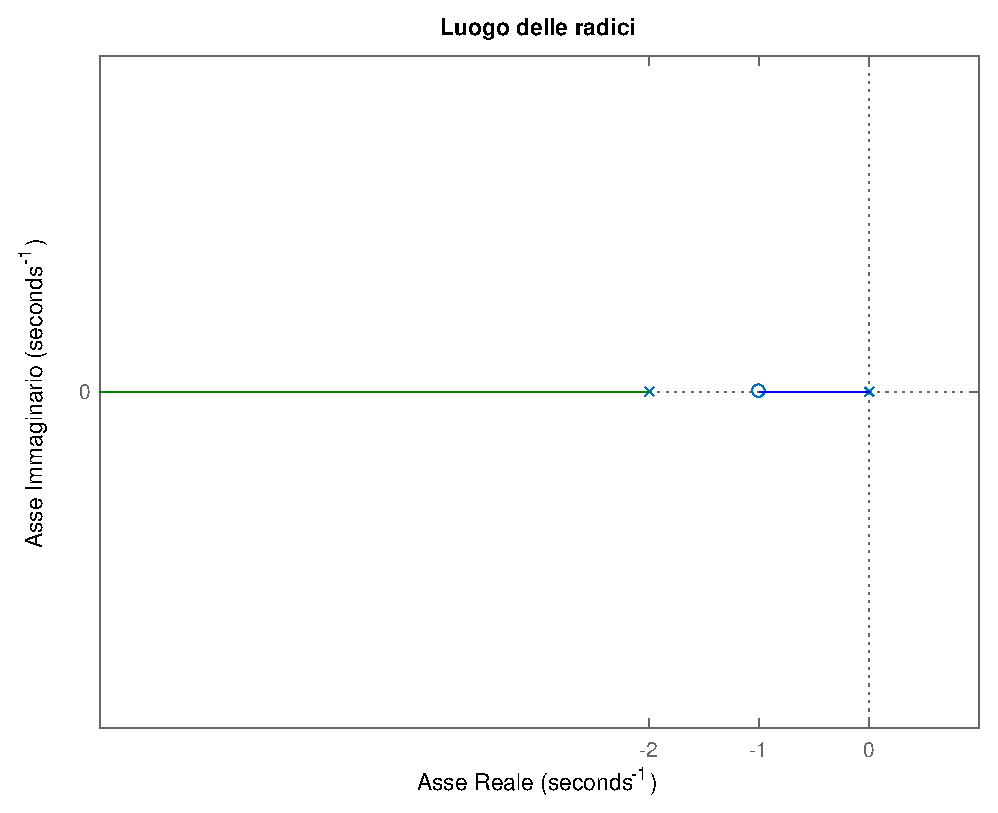
\includegraphics[scale=.6]{mod1/assets/rl_ex31}
\end{figure}

\begin{itemize}
	\item \emph{Punti di singolarità}:
		\begin{itemize}
			\item poli: \(\bigl\{-2, 0\bigr\}\)
			\item zeri: \(\bigl\{-1\bigr\}\)
		\end{itemize}
	\item \emph{Asintoti}:
		Determino centroide e angolo di inclinazione degli asintoti
		\[
			\sigma_a = \frac{0 -2 +1}{1} = -1
			\qquad
			\theta_a = \frac{\Bigl(2\cdot\bigl[0\bigr]+1\Bigr)\pi}{1} = \pi
		\]
	\item L'esercizio non richiede altro lavoro perché non presenta punti doppi,
		di intersezione con l'asse immaginario, etc.
	\item \emph{Stabilità}:
		\[\begin{cases}
			k = 0 & \text{sistema \emph{semplicemente stabile}} \\
			k > 0 & \text{sistema \emph{asintoticamente stabile}} \\
		\end{cases}\]
\end{itemize}


\exercise{}
Sia data la seguente funzione di trasferimento:
\[
	G(s) = \frac{s+1}{s^2}
\]
Determinare il luogo delle radici al variare di \(k > 0\).

\paragraph{Soluzione}

\begin{figure}[ht]
	\centering
	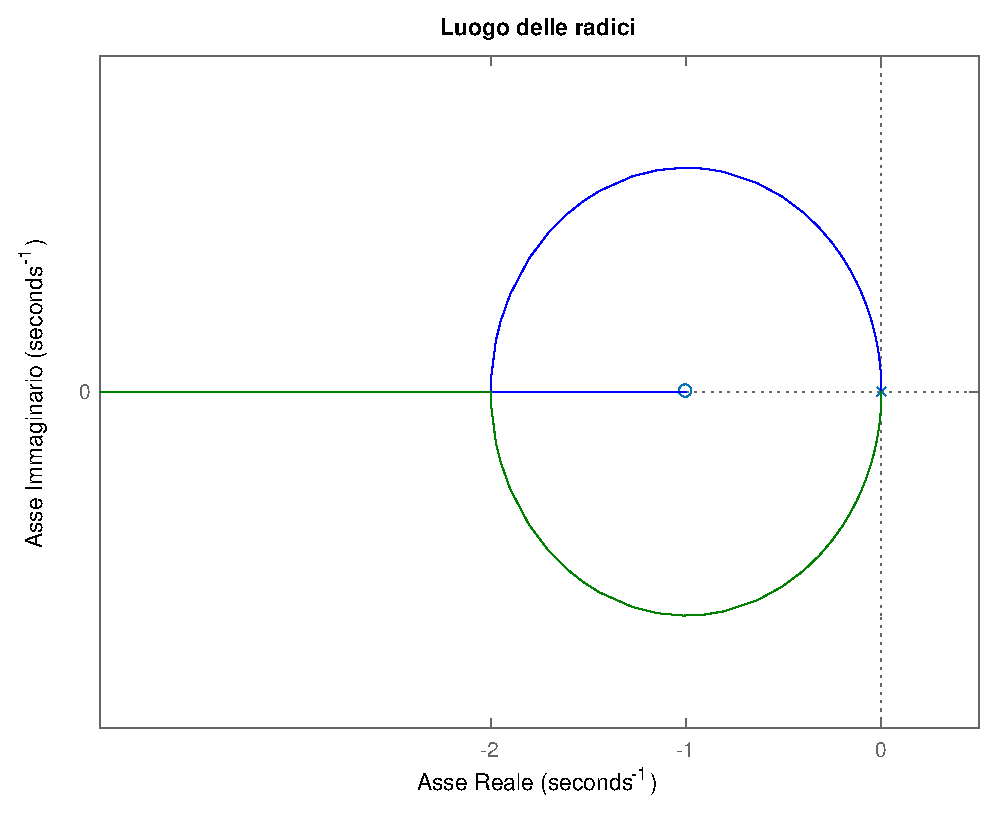
\includegraphics[scale=.6]{mod1/assets/rl_ex32}
\end{figure}

\begin{itemize}
	\item \emph{Punti di singolarità}:
		\begin{itemize}
			\item poli: \(\bigl\{ 0\,[\times 2] \bigr\}\)
			\item zeri: \(\bigl\{ -1 \bigr\}\)
		\end{itemize}
	\item \emph{Asintoti}:
		\[
			\sigma_a = \frac{0+1}{1} = 1 \qquad
			\theta_a = \frac{\Bigl(2\cdot\bigl[0\bigr]+1\Bigr)\pi}{1} = \pi
		\]
	\item Gli angoli di arrivo e di partenza sono entrambi di
		\(\pm \frac{\pi}{2}\), questo perché non sono punti complessi e
		coniugati.
	\item Posizione del punto di confluenza:
		\[
			G^\prime(s) = \frac{s^2 -2s(s+1)}{\cancel{s^4}} = 0
			\rightarrow s(s+2) = 0
			\implies s= \begin{cases} 0 \\ \bm{-2} \end{cases}
		\]
	\item Stabilità:
		\[\begin{cases}
			\text{Se } k = 0\colon & \text{sistema \emph{semplicemente stabile}} \\
			\text{Se } k > 0\colon & \text{sistema \emph{asintoticamente stabile}}
		\end{cases}\]
\end{itemize}


\exercise{}
Sia data la seguente funzione di trasferimento
\[
	G(s) = \frac{1}{s(s+1)(s+5)}
\]
Determinare il luogo delle radici al variare di \(k>0\).

\paragraph{Soluzione}

\begin{figure}[ht]
	\centering
	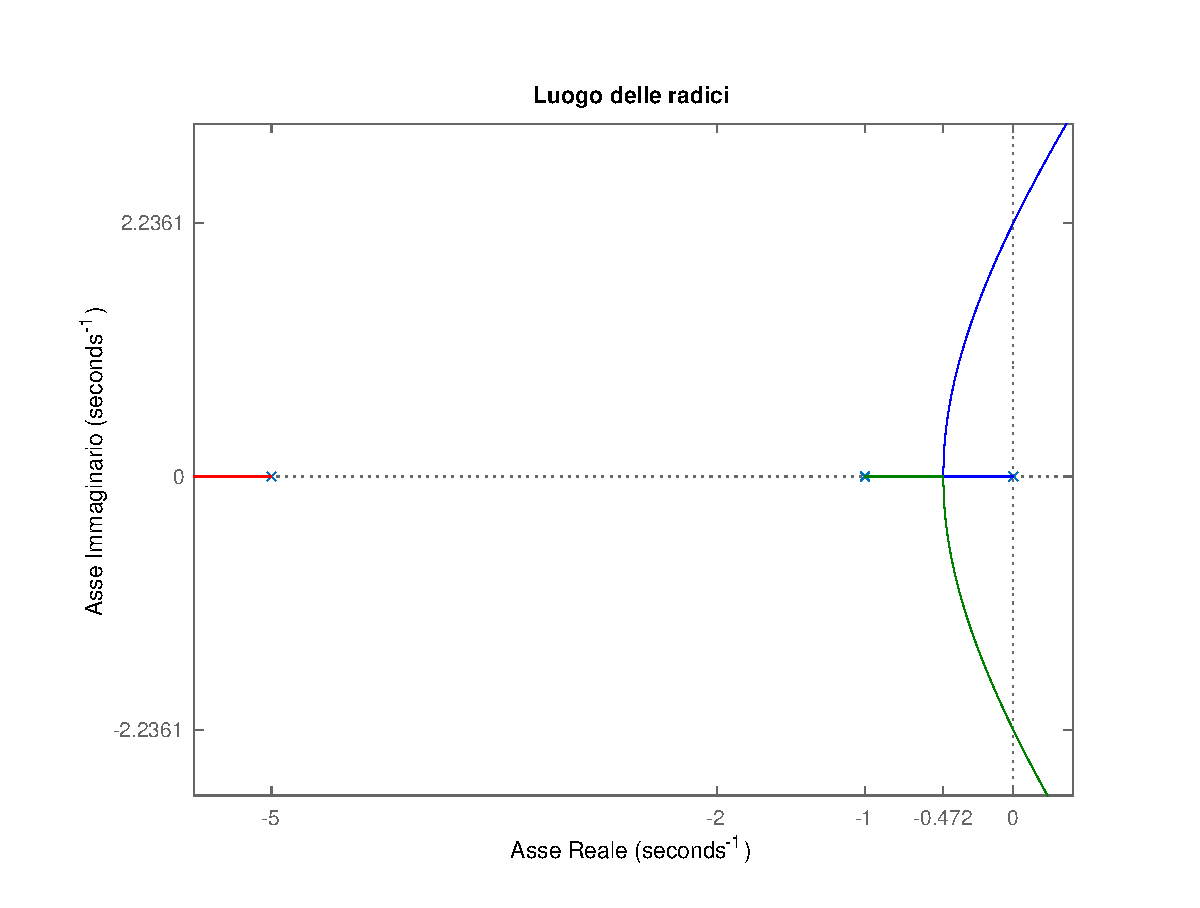
\includegraphics[scale=.6]{mod1/assets/rl_ex33}
\end{figure}

\begin{itemize}
	\item \emph{Punti di singolarità}:
		\begin{itemize}
			\item poli: \(\bigl\{ -5, -1, 0 \bigr\}\)
		\end{itemize}
	\item \emph{Asintoti}:
		\begin{align*}
			& \sigma_a = \frac{0-1-5}{3} = -2 \\
			& \theta_a = \frac{\Bigl( 2 \cdot \bigl[ 0, \dots, 2 \bigr] +1 \Bigr) \pi}{3} = \Bigl[ \frac{\pi}{3}, \pi, \frac{5}{3}\pi \Bigr]
		\end{align*}
	\item \emph{Punto doppio di emergenza}:
		\[
			G^\prime (s) = 0 \rightarrow -3s^2 -12s -5=0 \rightarrow s_{1,2} = \frac{-6\pm\sqrt{21}}{3} = \begin{cases} \bm{-0.472} \\ -3.527 \end{cases}
		\]
		Si sceglie il primo perché è il valore che appartiene al luogo delle radici.
	\item \emph{Punti di intersezione con l'asse immaginario}:
		applico il criterio di Routh per \(P(s) = s^3 +6s^2 +5s +k\):
		\[\begin{array}{r|rr}
			s^3      & 1 & 5 \\
			\bm{s^2} & 6 & k \\
			s^1      & \bm{30-k} \\
			s^0      & k
		\end{array}\]
		\[
			k = 30 \rightarrow 6s^2+30 = 0 \rightarrow s = \pm \jmath \sqrt{5}
		\]
	\item \emph{Stabilità}:
		\[\begin{cases}
			\text{Se } k = 0\colon & \text{sistema \emph{semplicemente stabile}} \\
			\text{Se } 0 < k < 30\colon & \text{sistema \emph{asintoticamente stabile}} \\
			\text{Se } k = 30\colon & \text{sistema \emph{semplicemente stabile}} \\
			\text{Se } k > 30\colon & \text{sistema \emph{instabile} con 2 poli instabili}
		\end{cases}\]
\end{itemize}


\exercise{}
Sia data la seguente funzione di trasferimento:
\[
	G(s) = \frac{(s+1.5)(s+4)}{s(s+1)(s+2.5)}
\]
Determinare il luogo delle radici per \(k>0\).

\paragraph{Soluzione}

\begin{figure}[ht]
	\centering
	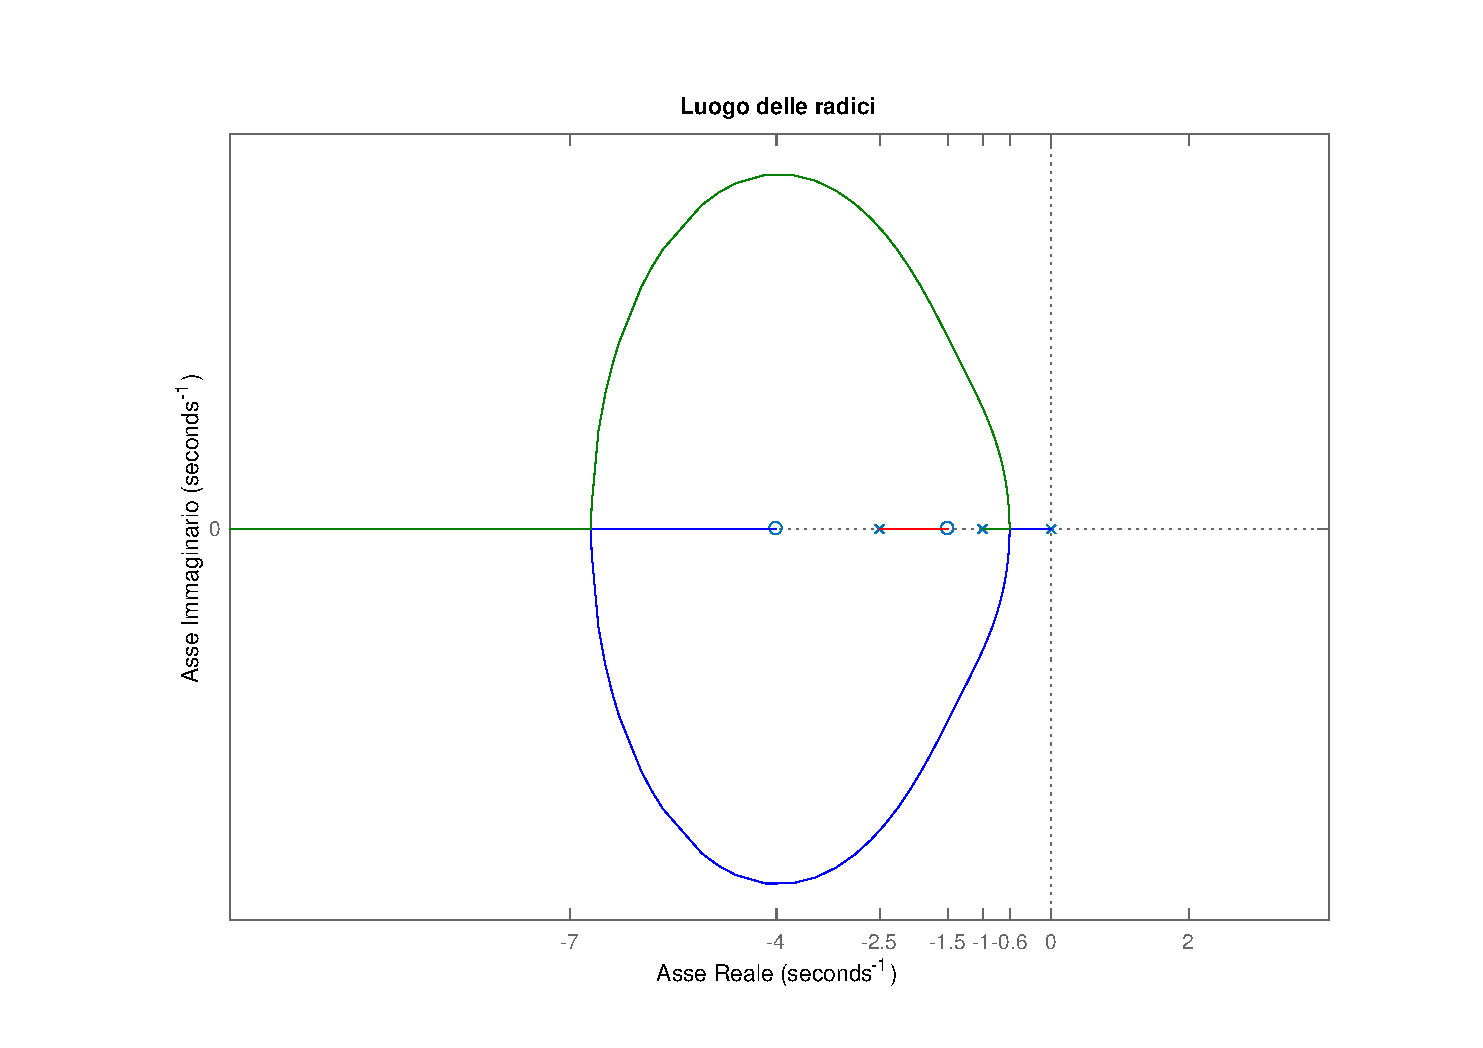
\includegraphics[scale=.6]{mod1/assets/rl_ex34}
\end{figure}

\begin{itemize}
	\item \emph{Punti di singolarità}:
		\begin{itemize}
			\item poli: \(\bigl\{ -2.5, -1, 0 \bigr\}\)
			\item zeri: \(\bigl\{ -4, -1.5 \bigr\}\)
		\end{itemize}
	\item \emph{Asintoti}:
		\begin{align*}
			& \sigma_a = \frac{0-1-2.5+1.5+4}{1} = 2 \\
			& \theta_a = \frac{\Bigl( 2 \cdot \bigl[0\bigr] +1 \Bigl)}{1} = \pi
		\end{align*}
	\item \emph{Punto doppio di emergenza}:
		lo ricavo con la tabella di taratura
		\[\begin{array}{rr}
			\toprule
			s & k \\
			\midrule
			-0.2 & 0.074 \\
			-0.4 & 0.127 \\
			\bm{-0.6} & \bm{0.149} \\
			-0.8 & 0.12 \\
			\bottomrule
		\end{array}\]
		Per \(s = -0.6\) si ha il massimo locale, ovvero il punto più
		approssimato al punto di emergenza.
	\item \emph{Punto doppio di confluenza}:
		\[\begin{array}{rr}
			\toprule
			s & k \\
			\midrule
			-5 & 14.286 \\
			-6 & 11.667 \\
			\bm{-7} & \bm{11.454} \\
			-8 & 11.846 \\
			\bottomrule
		\end{array}\]
		Per \(s = -7\) si ha il minimo locale, ovvero il più approssimato
		al punto di confluenza.
	\item \emph{Stabilità}:
		\[\begin{cases}
			k = 0\colon & \text{sistema \emph{semplicemente stabile}} \\
			k > 0\colon & \text{sistema \emph{asintoticamente stabile}}
		\end{cases}\]
\end{itemize}


\exercise{}
Sia data la seguente funzione di trasferimento:
\[
	G(s) = \frac{s+1}{s^2 (s+4)}
\]
Determinare il luogo delle radici per \(k>0\).

\paragraph{Soluzione}

\begin{figure}[ht]
	\centering
	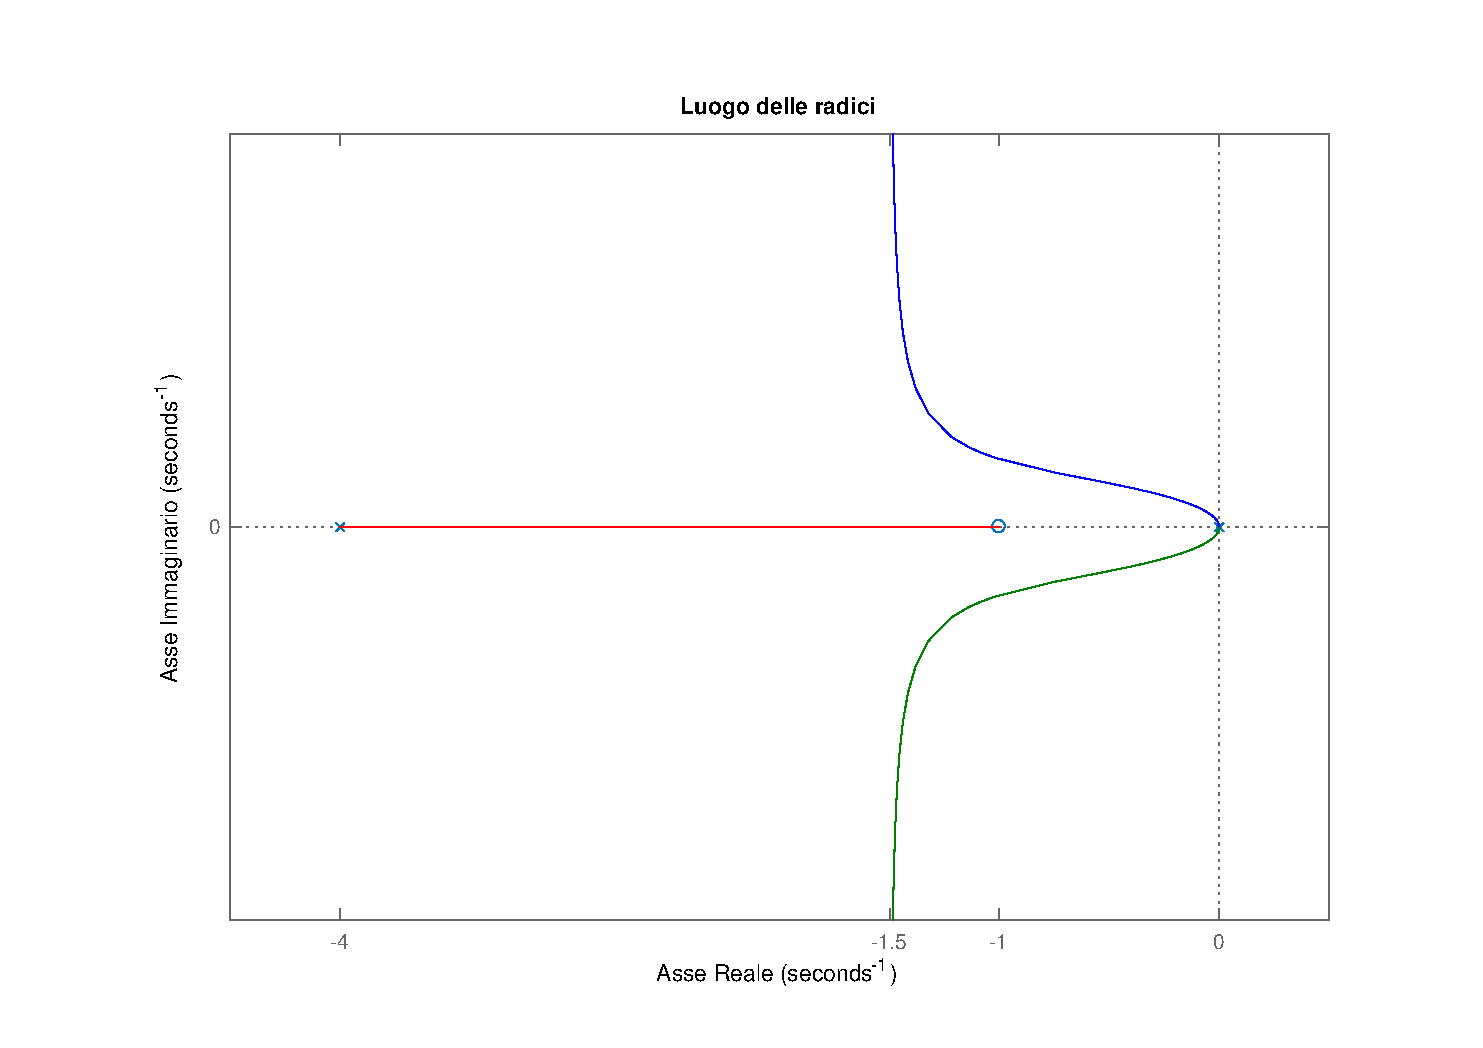
\includegraphics[scale=.6]{mod1/assets/rl_ex35}
\end{figure}

\begin{itemize}
	\item \emph{Punti di singolarità}:
		\begin{itemize}
			\item poli: \(\bigl\{ -4, 0\,[\times 2] \bigr\}\)
			\item zeri: \(\bigl\{ -1 \bigr\}\)
		\end{itemize}
	\item \emph{Asintoti}:
		\begin{align*}
			& \sigma_a = \frac{0-4+1}{2} = -\frac{3}{2} \\
			& \theta_a = \frac{\Bigl( 2 \cdot \bigl[ 0,1 \bigr] \pi \Bigr) \pi}{2} = \Bigl[ \frac{\pi}{2}, \frac{3}{2}\pi \Bigr]
		\end{align*}
	\item \emph{Angoli di partenza dei rami}: \(\frac{\pi}{2}\)
\end{itemize}


\exercise{}
Sia data la seguente funzione di trasferimento
\[
	G(s) = \frac{s+1}{s^2 (s+9)}
\]
Determinare il luogo delle radici per \(k>0\).

\paragraph{Soluzione}

\begin{figure}[ht]
	\centering
	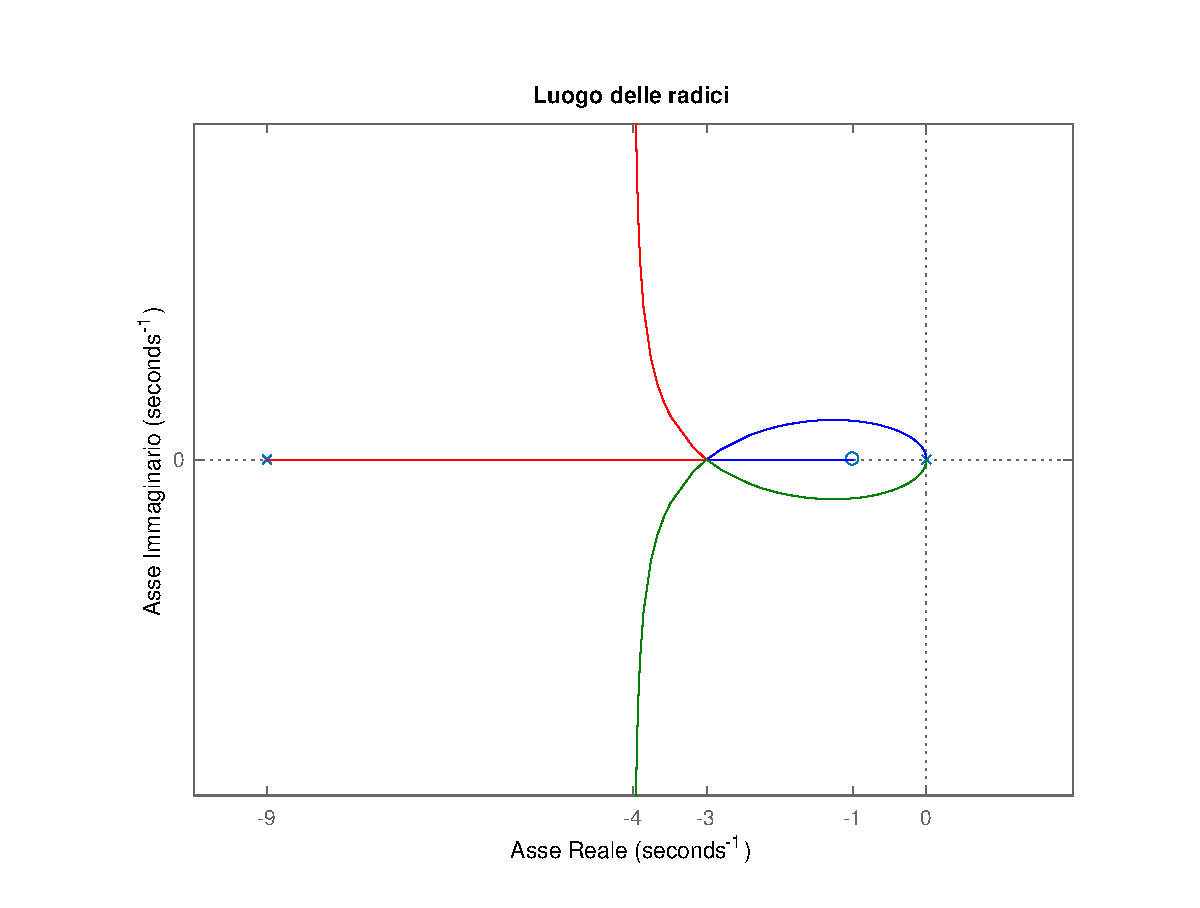
\includegraphics[scale=.6]{mod1/assets/rl_ex36}
\end{figure}

\begin{itemize}
	\item \emph{Punti di singolarità}:
		\begin{itemize}
			\item poli: \(\bigl\{ -9, 0\,[\times 2] \bigr\}\)
			\item zeri: \(\bigl\{ -1 \bigr\}\)
		\end{itemize}
	\item \emph{Asintoti}:
		\begin{align*}
			& \sigma_a = \frac{0-9+1}{2} = -4 \\
			& \theta_a = \frac{\Bigl(2 \cdot \bigl[ 0,1 \bigr] +1\Bigr) \pi}{2} = \Bigl[ \frac{\pi}{2}, \frac{3}{2}\pi \Bigr]
		\end{align*}
\end{itemize}
I poli all'origine si dirigono verso gli asintoti, ma sono soggetti all'attrazione
dello zero; quindi verifico possibili punti tripli nell'intervallo \((-4,-1)\):
\[
	G^\prime(s) = \frac{s^2(s+9) -\bigl(2s(s+9)+s^2\bigr)(s+1)}{\cancel{s^4 (s+9)^2}} = 0
	\rightarrow s(s+3)^2 = 0 \rightarrow s = \begin{cases} 0 \\ \bm{-3} \end{cases}
\]
Quindi si ha effettivamente un punto triplo in \(s = -3\), che impone la convergenza
dei rami che partono dai due poli all'origine e la loro emergenza verso gli asintoti.


\exercise{}
Sia data la seguente funzione di trasferimento:
\[
	G(s) = \frac{1}{s(s+2)\bigl( (s+1)^2 +4 \bigr)}
\]
Determinare il luogo delle radici per \(k>0\).

\paragraph{Soluzione}

\begin{figure}[ht]
	\centering
	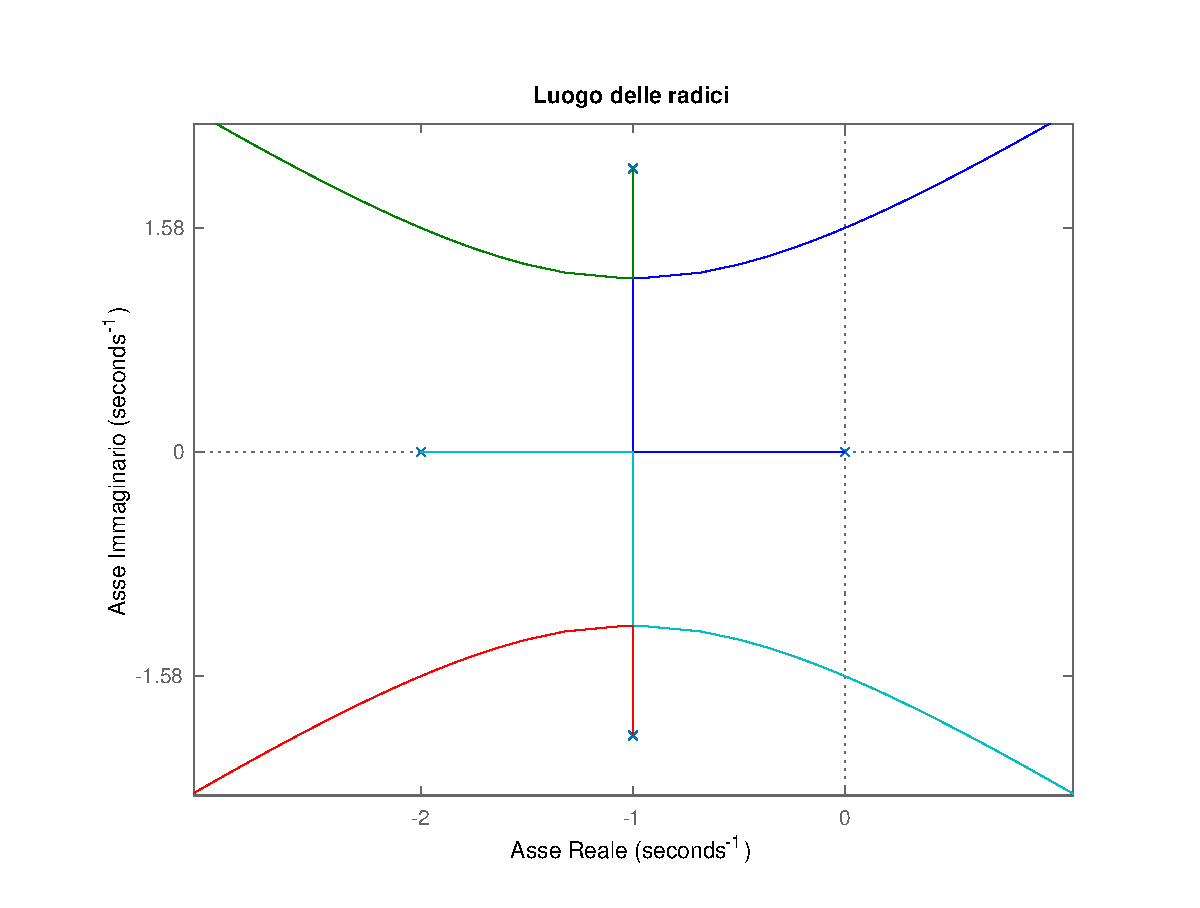
\includegraphics[scale=.6]{mod1/assets/rl_ex37}
\end{figure}

\begin{itemize}
	\item \emph{Punti di singolarità}:
		\begin{itemize}
			\item poli: \(\bigl\{ -2, -1\pm\jmath2, 0 \bigr\}\)
		\end{itemize}
	\item \emph{Asintoti}:
		\begin{align*}
			& \sigma_a = \frac{0-2-2(1\cancel{\pm\jmath2})}{4} = -1 \\
			& \theta_a = \frac{\Bigl(2 \cdot \bigl\{ 0,1,2,3 \bigr\} +1)\pi}{4} = \Bigl\{ \frac{\pi}{4}, \frac{3}{4}\pi, \frac{5}{4}\pi, \frac{7}{4}\pi \Bigr\}
		\end{align*}
	\item \emph{Punti doppi}:
		calcolando \(G^\prime(s) = 0\) si ottiene l'equazione
		\[
			2s^3 +6s^2 +9s +5 = 0 \rightarrow s = \begin{cases} -1 \\ -1 \pm\jmath\sqrt{\frac{3}{2}} \end{cases}
		\]
		Questo significa che ci sono 3 punti doppi dove i poli si
		''scontrano'' e così si diramano.
	\item \emph{Angoli di partenza} per i poli complessi e coniugati:
		\begin{align*}
			\varphi_+ &= \pi - \angle(-1+\jmath2) -\angle(-1+\jmath2+2) -\angle(\cancel{-1}+\jmath2\cancel{+1}+\jmath2) = \\
				  &= \pi +\arctan{2} -\pi -\arctan{2} -\frac{\pi}{2} = -\frac{\pi}{2} \\
			\varphi_- &= \pi -\angle(-1-\jmath2) -\angle(-1-\jmath2+2) -\angle(\cancel{-1}-\jmath2\cancel{+1}-\jmath2) = \\
				  &= \pi +\arctan{2} -\pi -\arctan{2} +\frac{\pi}{2} = \frac{\pi}{2}
		\end{align*}
	\item \emph{Intersezioni con l'asse immaginario}:
		\[
			P(s) = s^4 +4s^3 +9s^2 +10s +k
		\]
		\[
			\begin{array}{r|rrr}
				s^4 & 1 &  9 & k \\
				s^3 & 4 & 10 \\
				\bm{s^2} & \cancelto{13}{26} & \cancelto{2}{4} k \\
				s^1 & \bm{65-4k} \\
				s^0 & 2k
			\end{array}
		\]
		Per \(k = \frac{65}{4} = \frac{13\cdot5}{4} \rightarrow \cancel{13}s^2 + \frac{\cancel{13}\cdot5}{2} = 0 \rightarrow s = \pm\jmath\sqrt{\frac{5}{2}}\)
	\item \emph{Stabilità}:
		\[\begin{cases}
			k=0\colon & \text{sistema \emph{semplicemente stabile}} \\
			0<k<\frac{65}{4}\colon & \text{sistema \emph{asintoticamente stabile}} \\
			k=\frac{65}{4}\colon & \text{sistema \emph{semplicemente stabile}} \\
			k>\frac{65}{4}\colon & \text{sistema \emph{instabile} con 2 poli instabili}
		\end{cases}\]
\end{itemize}


\exercise{}
Sia data la seguente funzione di trasferimento:
\[
	G(s) = \frac{1}{s(s+1)(s+3)(s+4)}
\]
Determinare il luogo delle radici per \(k>0\) e \(k<0\).

\paragraph{Soluzione per \(k > 0\)}

\begin{figure}[ht]
	\centering
	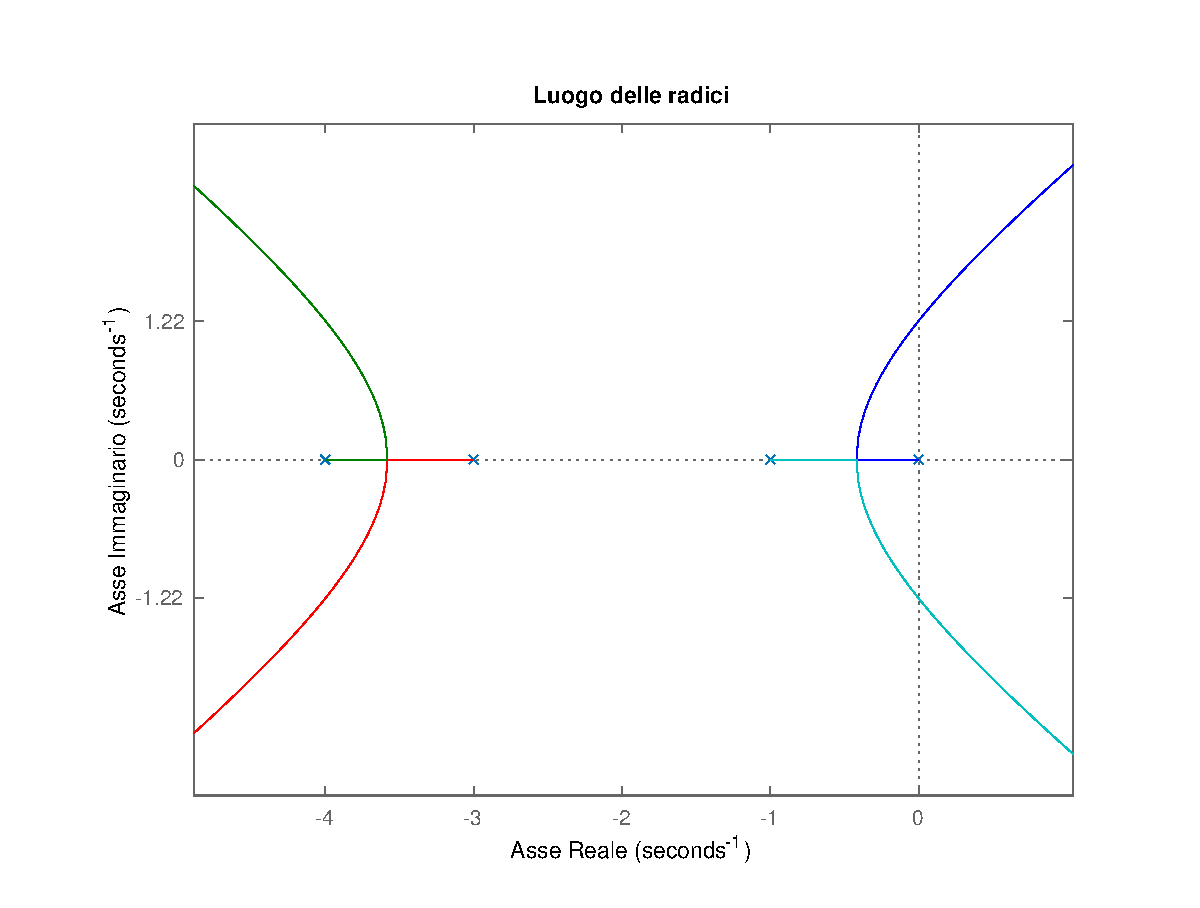
\includegraphics[scale=.6]{mod1/assets/rl_ex38}
\end{figure}

\begin{itemize}
	\item \emph{Punti di singolarità}:
		\begin{itemize}
			\item poli: \(\bigl\{ -4,-3,-1,0 \bigr\}\)
		\end{itemize}
	\item \emph{Asintoti}:
		\begin{align*}
			& \sigma_a = \frac{0-1-3-4}{4} = -2 \\
			& \theta_a = \frac{\Bigl(2\cdot\bigl[0,1,2,3\bigr]+1\Bigr)\pi}{4} = \Bigl[ \frac{\pi}{4},\frac{3}{4}\pi,\frac{5}{4}\pi,\frac{7}{4}\pi \Bigr]
		\end{align*}
	\item \emph{Punti doppi}: \(k = -s(s+1)(s+3)(s+4)\)
		\[\begin{array}{rr}
			\toprule
			s 	  & k 		\\
			\midrule
			-0.3 	  & 2.098 	\\
			\bm{-0.5} & \bm{2.187}	\\
			-0.7 	  & 1.594	\\
			\bottomrule
		\end{array}\]
		\(s=-0.5\) è un punto doppio di emergenza.
		\[\begin{array}{rr}
			\toprule
			s 	  & k 		\\
			\midrule
			-3.3 	  & 1.594 	\\
			\bm{-3.5} & \bm{2.187} 	\\
			-3.7 	  & 2.098 	\\
			\bottomrule
		\end{array}\]
		\(s=-3.5\) è un punto doppio di emergenza.
	\item \emph{Intersezioni con l'asse immaginario}:
		\[
			P(s) = s^4 +8s^3 +19s^2 +12s +k
		\]
		\[\begin{array}{r|rrr}
			s^4 	 &  1 & 19 & k  \\
			s^3 	 &  8 & 12 	\\
			\bm{s^2} & 35 & 2k 	\\
			s^1 	 & \bm{105-4k} 	\\
			s^0 	 & 2k
		\end{array}\]
		\(k = \frac{105}{4} = \frac{35\cdot3}{4} \rightarrow s^2+\frac{3}{2} = 0 \rightarrow s = \pm\jmath\sqrt{\frac{3}{2}}\)
	\item \emph{Stabilità}:
		\[\begin{cases}
			k = 0\colon & \text{sistema \emph{semplicemente stabile}} \\
			0<k<\frac{105}{4}\colon & \text{sistema \emph{asintoticamente stabile}} \\
			k = \frac{105}{4}\colon & \text{sistema \emph{semplicemente stabile}} \\
			k > \frac{105}{4}\colon & \text{sistema \emph{instabile} con 2 poli instabili}
		\end{cases}\]
\end{itemize}

\paragraph{Soluzione per \(k < 0\)}

\begin{figure}[ht]
	\centering
	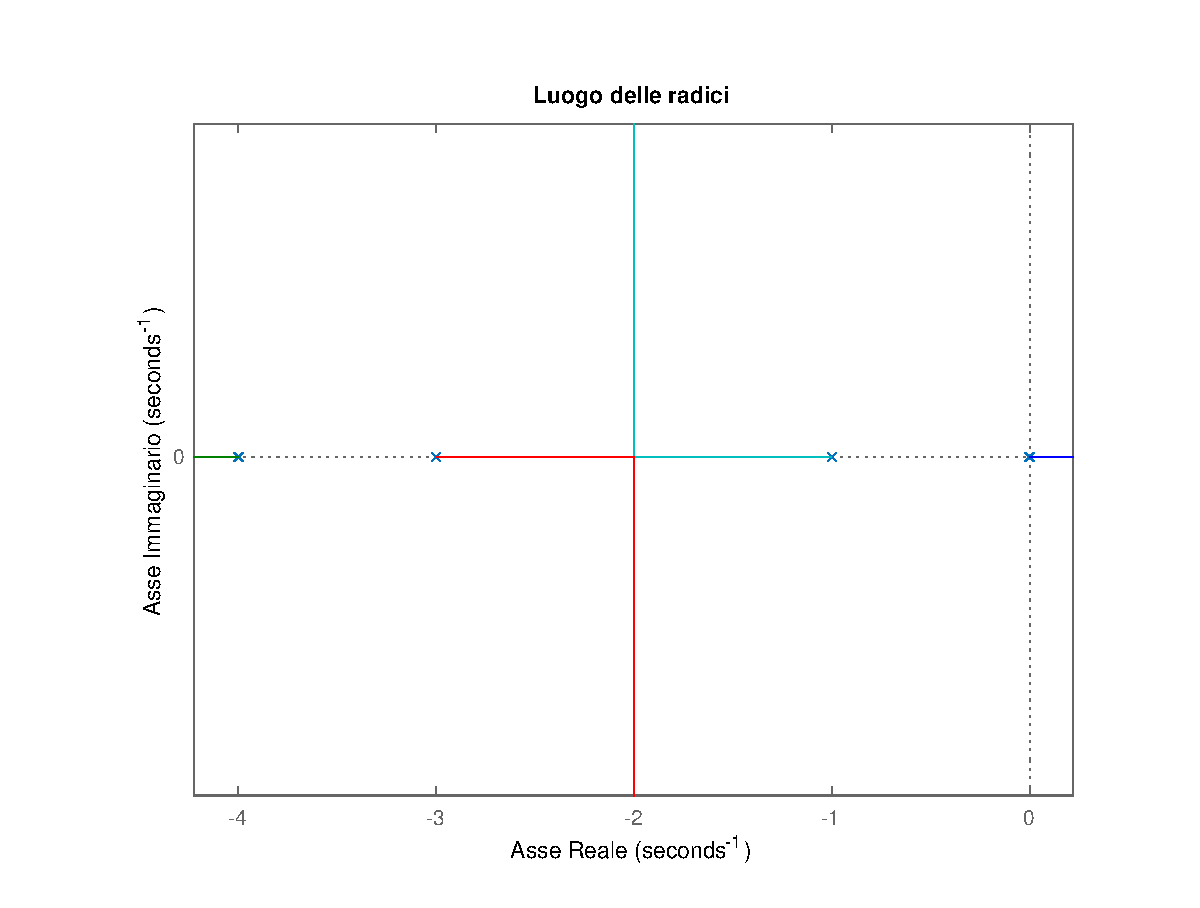
\includegraphics[scale=.6]{mod1/assets/rl_ex38n}
\end{figure}

\begin{itemize}
	\item \emph{Asintoti}:
		\[
			\sigma_a = -2 \qquad \theta_a = \frac{2\cdot\bigl[ 0,1,2,3 \bigr]\pi}{4} = \Bigl[ 0,\frac{\pi}{2},\pi,\frac{3}{2}\pi \Bigr]
		\]
	\item \emph{Stabilità}: per \(k < 0\) il sistema è \emph{instabile} con 1 polo instabile.
\end{itemize}

\paragraph{Determinare i poli per i punti critici}
\[\begin{cases}
	k = 0\colon & \bigl\{ -4,-3,-1,0 \bigr\} \\
	k = \frac{105}{4}\colon & \begin{cases}
		\text{2 poli puramente immaginari: } s_{1,2} = \pm\jmath\sqrt{\frac{3}{2}} \\
		\text{2 poli stabili: } s_{3,4} = -4 \pm\jmath\sqrt{\frac{3}{2}}
	\end{cases}
\end{cases}\]


\exercise{}
Sia data la seguente funzione di trasferimento:
\[
	G(s) = \frac{s-1}{(s+2)(s-2)(s+4)}
\]
Determinare il luogo delle radici per \(k\in\mathbb{R}^2\).

\paragraph{Soluzione}

\begin{figure}[ht]
	\centering
	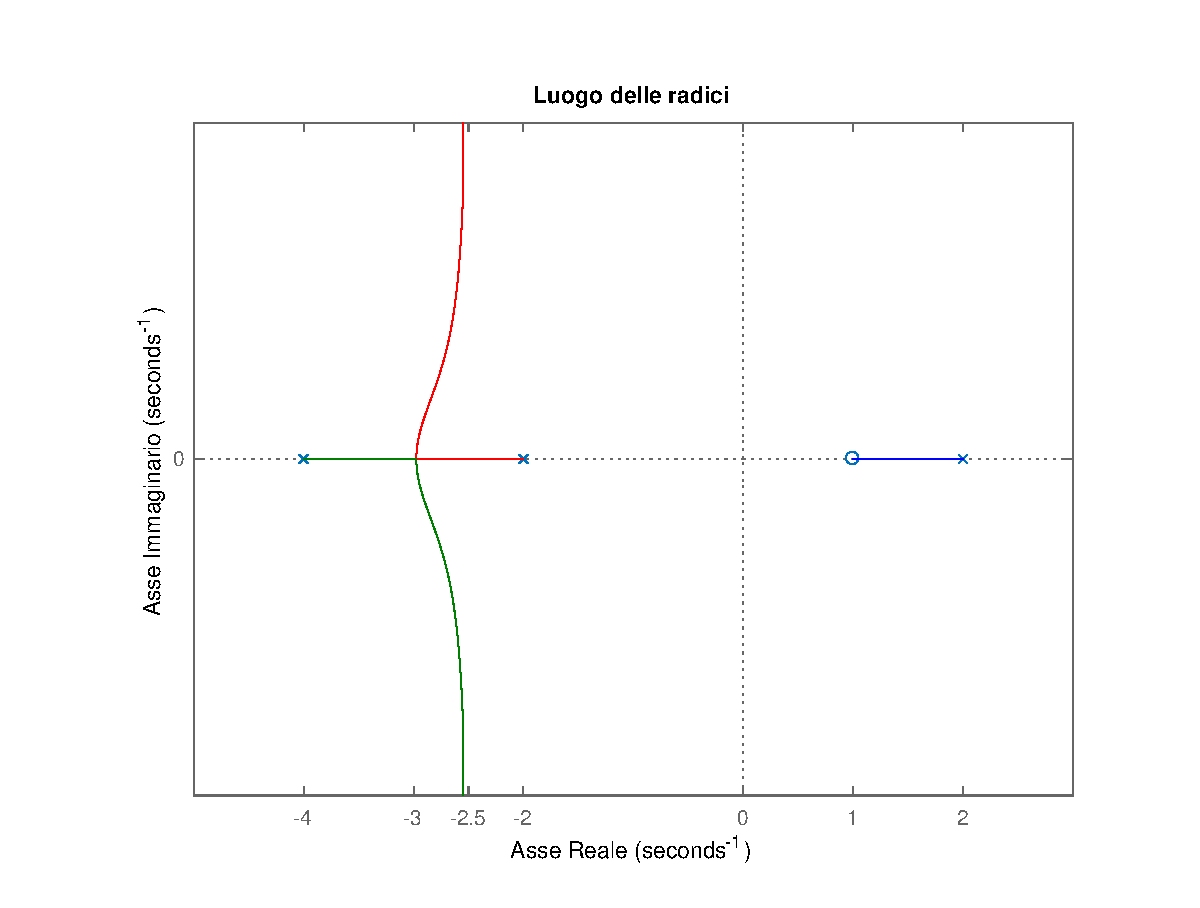
\includegraphics[scale=.6]{mod1/assets/rl_ex39}
\end{figure}

\begin{itemize}
	\item \emph{Punti di singolarità}:
		\begin{itemize}
			\item poli: \(\bigl\{ -4,-2,2 \bigr\}\) \\
			\item zeri: \(\bigl\{ 1 \bigr\}\)
		\end{itemize}
	\item \emph{Asintoti}:
		\[
			\sigma_a = \frac{-2+2-4-1}{2} = -\frac{5}{2} \qquad
			\theta_a = \frac{\Bigl(2\cdot \bigl[0,1\bigr] +1\Bigr)\pi}{2} = \Bigl[ \frac{\pi}{2},\frac{3}{2}\pi \Bigr]
		\]
	\item \emph{Punti doppi}:
		\[
			k = -\frac{1}{G(s)} = + \frac{(s+2)(s-2)(s+4)}{1-s} \quad
			\text{per } s \in \Bigl(-4,-2\Bigr)
		\]
		\[\begin{array}{rr}
			\toprule
			s 	  & k 		\\
			\midrule
			-3.5 	  & 0.917 	\\
			-3.3 	  & 1.123 	\\
			\bm{-3.0} & \bm{1.25} 	\\
			-2.7 	  & 1.156	\\
			\bottomrule
		\end{array}\]
		Per \(s=-3\) si ha un punto doppio di emergenza.
	\item \emph{Stabilità}: il sistema è sempre \emph{instabile} con 1 polo instabile.
\end{itemize}


\exercise{}
Siano dati
\[
	G_p(s) = \frac{s+1}{s(s-5)(s+5)} \qquad G_c(s) = k
\]
Determinare il luogo delle radici del sistema ad anello chiuso per \(k>0\).

\paragraph{Soluzione}

Si ricorda che
\begin{center}\begin{tikzpicture}[auto,node distance=2cm,>=latex']
	\node [input] (x) {};
	\node [sum, right of=x] (sum) {};
	\node [block, right of=sum] (B) {\(G_c(s)\)};
	\node [block, right of=B] (D) {\(G_p(s)\)};
	\node [tmp, right of=D] (tmp) {};
	\node [output, right of=tmp] (y) {};
	\draw [->] (x) -- node[pos=0]{\(x\)} (sum);
	\draw [->] (sum) -- (B) -- node[pos=0.5,name=achr]{} (D) -- (tmp) -- node[pos=1]{\(y\)} (y);
	\node [block, below of=achr, node distance=1.5cm] (C) {\(H(s)\)};
	\draw [->] (tmp) |- (C) -| node[pos=0.9,anchor=west]{\(-\)} (sum);
\end{tikzpicture}\end{center}
Quindi si ha \(G(s)H(s) = G(s)\) considerando \(H(s)\) unitario.

\begin{figure}[ht]
	\centering
	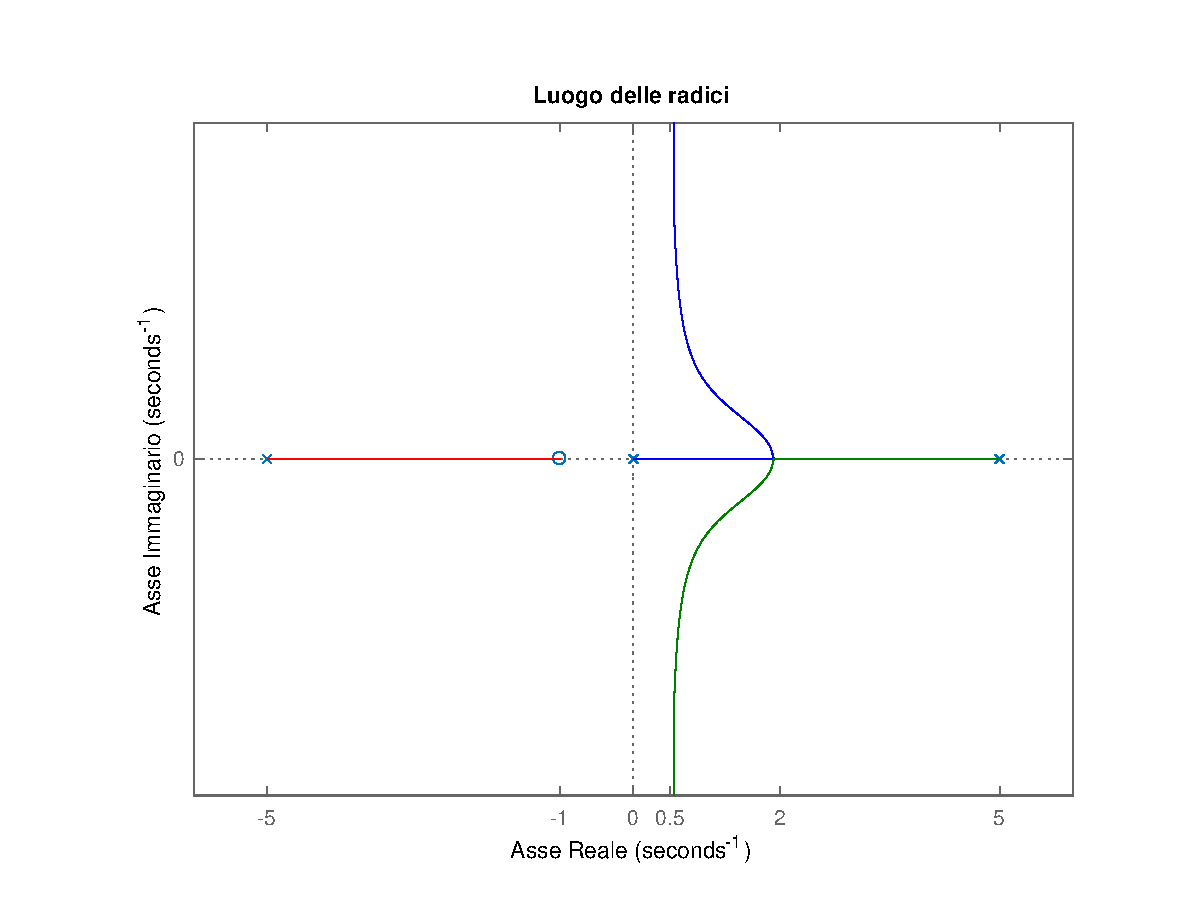
\includegraphics[scale=.6]{mod1/assets/rl_ex310}
\end{figure}

\begin{itemize}
	\item \emph{Punti di singolarità}:
		\begin{itemize}
			\item poli: \(\bigl\{ -5,0,5 \bigr\}\)
			\item zeri: \(\bigl\{ -1 \bigr\}\)
		\end{itemize}
	\item \emph{Asintoti}:
		\[
			\sigma_a = \frac{0+5-5+1}{2} = \frac{1}{2} \qquad
			\theta_a = \frac{\Bigl(2\cdot \bigl[0,1\bigr]\Bigr)\pi}{2} = \Bigl[ \frac{\pi}{2},\frac{3}{2}\pi \Bigr]
		\]
	\item \emph{Punti doppi}:
		\[
			k = -\frac{1}{G(s)} = -\frac{s(s-5)(s+5)}{s+1} \quad
			\text{per } s \in \Bigl( \frac{1}{2},5 \Bigr)
		\]
		\[\begin{array}{rr}
			\toprule
			s 	&       k \\
			\midrule
			1 	&      12 \\
			1.5 	&   13.65 \\
			\bm{2} 	& \bm{14} \\
			2.5 	&   13.39 \\
			\bottomrule
		\end{array}\]
		Per \(s=-2\) si ha un punto doppio di emergenza.
	\item \emph{Stabilità}: per \(k \geq 0\) il sistema è \emph{instabile}
		con 2 poli instabili.
\end{itemize}


\exercise{}
Sia data la seguente funzione di trasferimento:
\[
	G(s) = \frac{s-1}{s^2(s^2+4s+8)}
\]
Determinare il luogo delle radici per \(k>0\) e \(k<0\).

\paragraph{Soluzione per \(k>0\)}
È possibile semplificare \(G(s)\) per rendere noti i poli coniugati e complessi:
\[
	G(s) = \frac{s-1}{s^2\bigl( (s+2)^2 +4 \bigr)}
\]

\begin{figure}[ht]
	\centering
	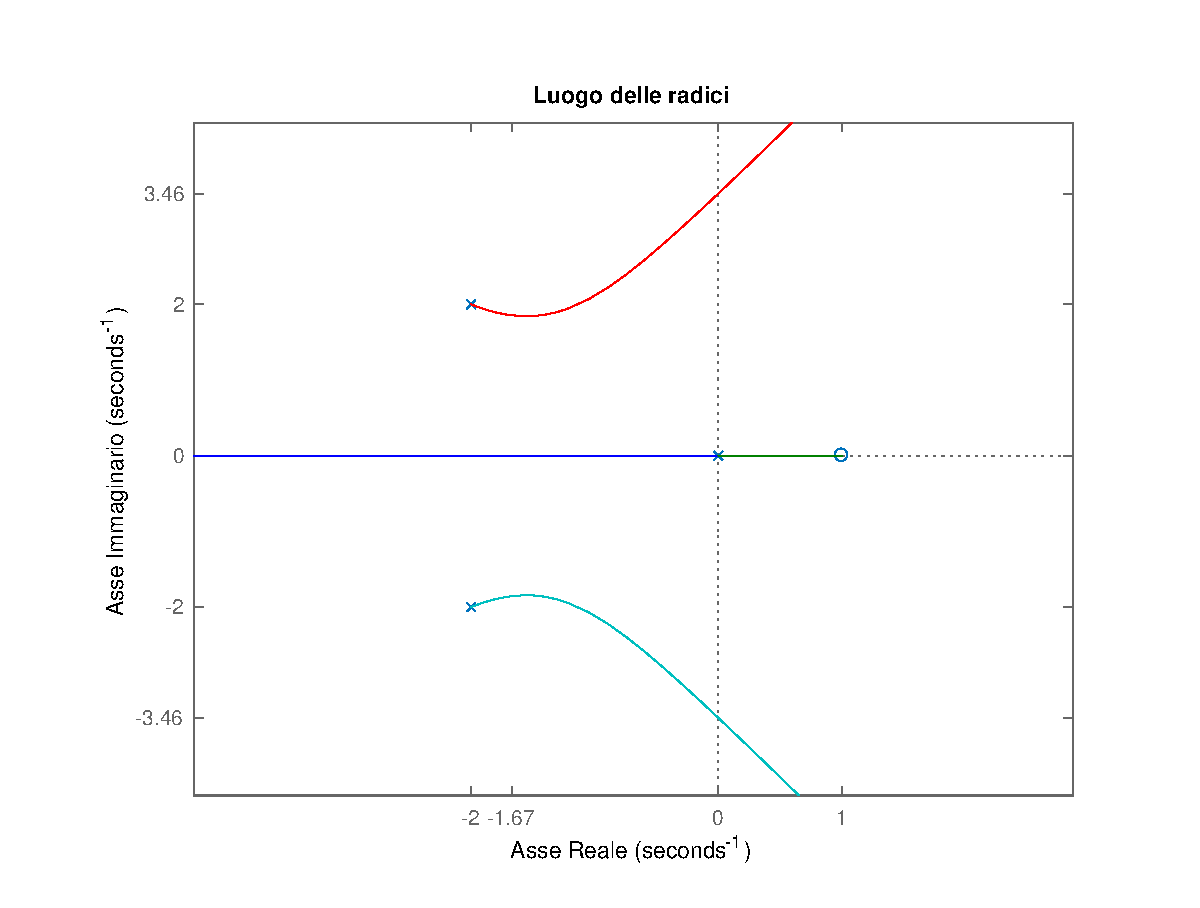
\includegraphics[scale=.5]{mod1/assets/rl_ex311}
	\caption{per \(k>0\)}
\end{figure}

\begin{itemize}
	\item \emph{Punti di singolarità}:
		\begin{itemize}
			\item poli: \(\bigl\{ -2\pm\jmath2, 0\,[\times 2] \bigr\}\)
			\item zeri: \(\bigl\{ 1 \bigr\}\)
		\end{itemize}
	\item \emph{Asintoti}:
		\[
			\sigma_a = \frac{0-4\pm\jmath2-1}{3} = -\frac{5}{3} \qquad
			\theta_a = \frac{\Bigl(2\cdot \bigl[ 0,1,2 \bigr] +1 \Bigr)\pi}{3} = \Bigl[ \frac{\pi}{3},\pi,\frac{5}{3}\pi \Bigr]
		\]
	\item \emph{Intersezioni con l'asse immaginario}:
		\[
			P(s) = s^4 +4s^3 +8s^2 +ks -k
		\]
		\[\begin{array}{r|rrr}
			s^4 	 & 1    &   8 & -k \\
			s^3 	 & 4    &   k 	   \\
			\bm{s^2} & 32-k & -4k 	   \\
			s^1 	 & \bm{48-k} 	   \\
			s^0 	 & -4k
		\end{array}\]
		Per \(k = 48 = 16\cdot3\) si ha \(-16s^2-16\cdot12=0 \rightarrow
		s = \pm\jmath2\sqrt{3}\).
	\item \emph{Angoli di partenza} per \(s = -2\pm\jmath2\):
		\begin{align*}
			\varphi_- &= \pi + \angle(-2-\jmath2-1) -\angle(-2-\jmath2+2-\jmath2) -2\angle(-2-\jmath2-0) = \\
				  &= \pi + \arctan{\frac{2}{3}} -\pi +\frac{\pi}{2} -2\arctan{1} +2\pi = \\
				  &= 2\pi +0.588 +\frac{\pi}{2} -2\frac{\pi}{4} = \SI{0.588}{\radian} \\
			\varphi_+ &= \pi +\angle(-2+\jmath2-1) -\angle(-2+\jmath2+2+\jmath2) -2\angle(-2+\jmath2-0) = \\
				  &= \pi +\arctan{-\frac{2}{3}} +\pi -\frac{\pi}{2} -2\arctan{-1} -2\pi = \\
				  &= -0.588 -\frac{\pi}{2} -2\frac{\pi}{4} = \SI{-0.588}{\radian}
		\end{align*}
	\item \emph{Stabilità}:
		\[\begin{cases}
			k = 0\colon & \text{sistema \emph{semplicemente stabile}} \\
			0 < k \leq 48\colon & \text{sistema \emph{instabile} con 1 polo instabile} \\
			k > 48\colon & \text{sistema \emph{instabile} con 3 poli instabili}
		\end{cases}\]
\end{itemize}

\paragraph{Soluzione per \(k<0\)}

\begin{figure}[ht]
	\centering
	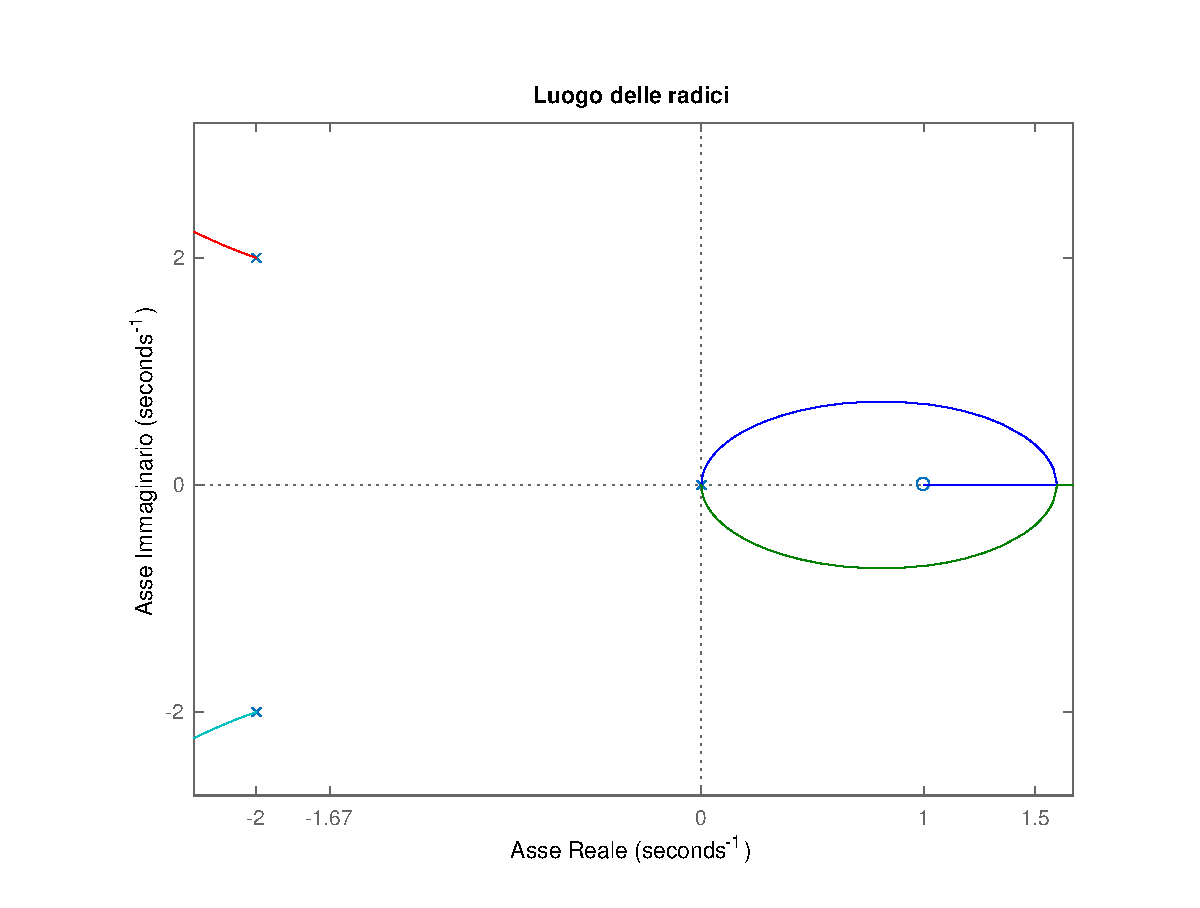
\includegraphics[scale=.5]{mod1/assets/rl_ex311n}
	\caption{per \(k<0\)}
\end{figure}

\begin{itemize}
	\item \emph{Asintoti}:
		\[
			\sigma_a = -\frac{5}{3} \qquad
			\theta_a = \frac{\Bigl(2\cdot\bigl[0,1,2\bigr]\Bigr)\pi}{3} = \Bigl[0,\frac{2}{3}\pi,\frac{4}{3}\pi\Bigr]
		\]
	\item \emph{Punti doppi}:
		\[
			k = -\frac{s^2\bigl((s+2)^2+4\bigr)}{s-1} \quad
			\text{per } s \in (1,+\infty)
		\]
		\[\begin{array}{rr}
			\toprule
			s 	 & k 		\\
			\midrule
			1.3 	 & -83.88 	\\
			\bm{1.5} & \bm{-73.12} \\
			2 	 & -80 		\\
			\bottomrule
		\end{array}\]
		Per \(s=1.5\) si ha un punto doppio di \emph{confluenza}.
	\item \emph{Stabilità}: per \(k<0\) il sistema è \emph{instabile} con
		2 poli instabili.
\end{itemize}


\exercise{}
Sia data la seguente funzione di trasferimento:
\[
	G(s) = \frac{s+4}{s(s^2+2s+2)}
\]
Determinare il luogo delle radici per \(k>0\).

\paragraph{Soluzione}

\begin{figure}[ht]
	\centering
	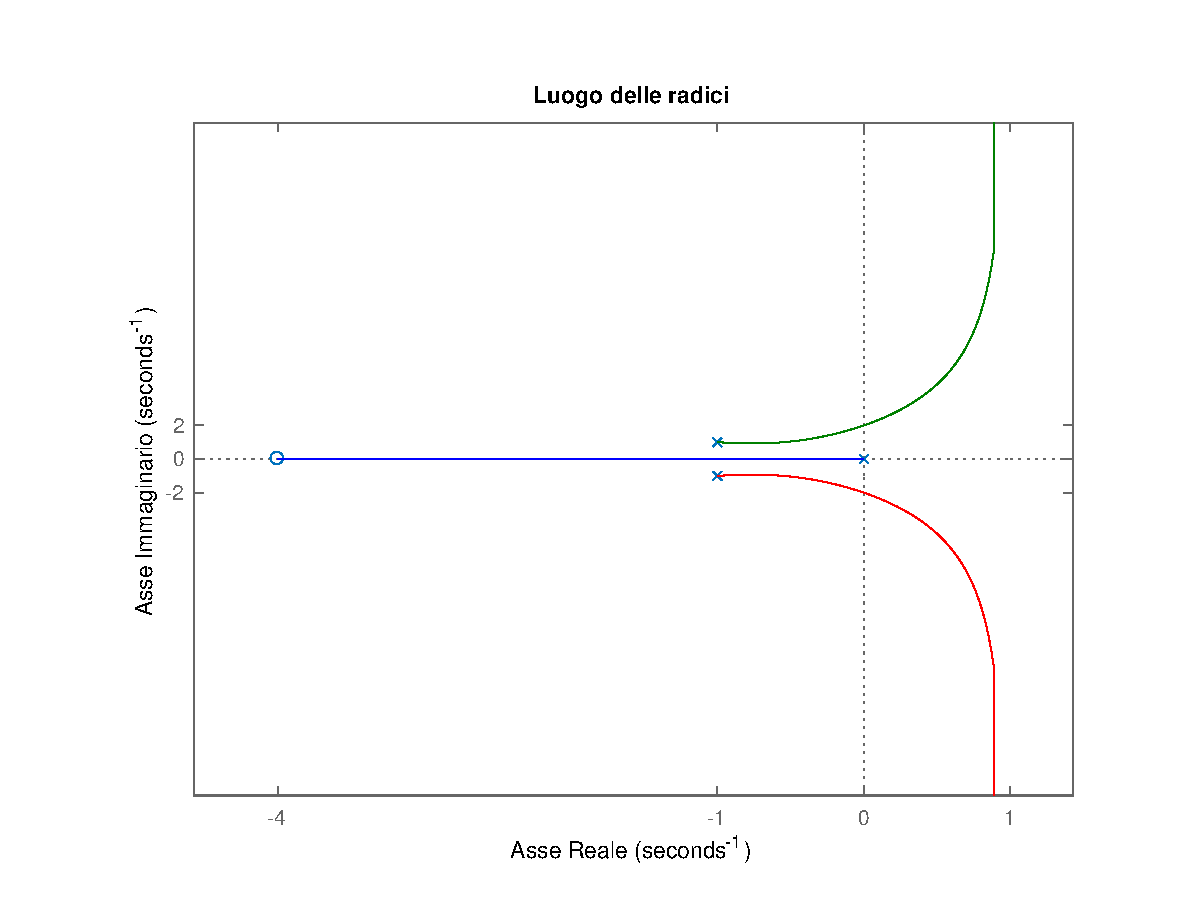
\includegraphics[scale=.6]{mod1/assets/rl_ex312}
\end{figure}

\begin{itemize}
	\item \emph{Punti di singolarità}:
		\begin{itemize}
			\item poli: \(\bigl\{-1\pm\jmath,0\bigr\}\)
			\item zeri: \(\bigl\{-4\bigr\}\)
		\end{itemize}
	\item \emph{Asintoti}:
		\[
			\sigma_a = \frac{-2\pm\jmath+4}{2} = 1 \qquad
			\theta_a = \frac{\Bigl(2\cdot\bigl[0,1\bigr]+1\Bigr)\pi}{2} = \Bigl[\frac{\pi}{2},\frac{3}{2}\pi\Bigr]
		\]
	\item \emph{Intersezioni con l'asse immaginario}:
		\[
			P(s) = s^3 + 2s^2 +(2+k)s +4k
		\]
		\[\begin{array}{r|rr}
			s^3 & 1 & 2+k 	   \\
			\bm{s^2} & 2 & 4k  \\
			s^1 & \bm{2-k} 	   \\
			s^0 & 4k
		\end{array}\]
		Per \(k=2\): \(2s^2+8=0 \rightarrow s=\pm\jmath2\)
	\item \emph{Angoli di partenza} per \(s=-1\pm\jmath\):
		\begin{align*}
			\varphi_- &= \pi +\angle(-1-\jmath+4) -\angle(-1-\jmath+1-\jmath) -\angle(-1-\jmath) = \\
				  &= \pi +\arctan{-\frac{1}{3}} +\frac{\pi}{2} -\arctan{1} +\pi = \\
				  &= 2\pi +\frac{\pi}{2} -0.322 -\frac{\pi}{4} = \SI{0.463}{\radian} \\
			\varphi_+ &= \pi +\angle(-1+\jmath+4) -\angle(-1+\jmath+1+\jmath) -\angle(-1+\jmath) = \\
				  &= \pi +\arctan{\frac{1}{3}} -\frac{\pi}{2} -\arctan{-1} -\pi = \\
				  &= -\frac{\pi}{2} +\frac{\pi}{4} +0.322 = \SI{-0.463}{\radian}
		\end{align*}
	\item \emph{Stabilità}:
		\[\begin{cases}
			k = 0\colon & \text{sistema \emph{semplicemente stabile}} \\
			0 < k < 2\colon & \text{sistema \emph{asintoticamente stabile}} \\
			k = 2\colon & \text{sistema \emph{semplicemente stabile}} \\
			k > 2\colon & \text{sistema \emph{instabile} con 2 poli instabili}
		\end{cases}\]
\end{itemize}

\exercise{}
Sia data la seguente funzione di trasferimento:
\[
	G(s) = \frac{s-6}{s(s^2+4s+13)}
\]
Determinare il luogo delle radici per \(k>0\) e \(k<0\).

\paragraph{Soluzione per \(k>0\)}

\begin{figure}[ht]
	\centering
	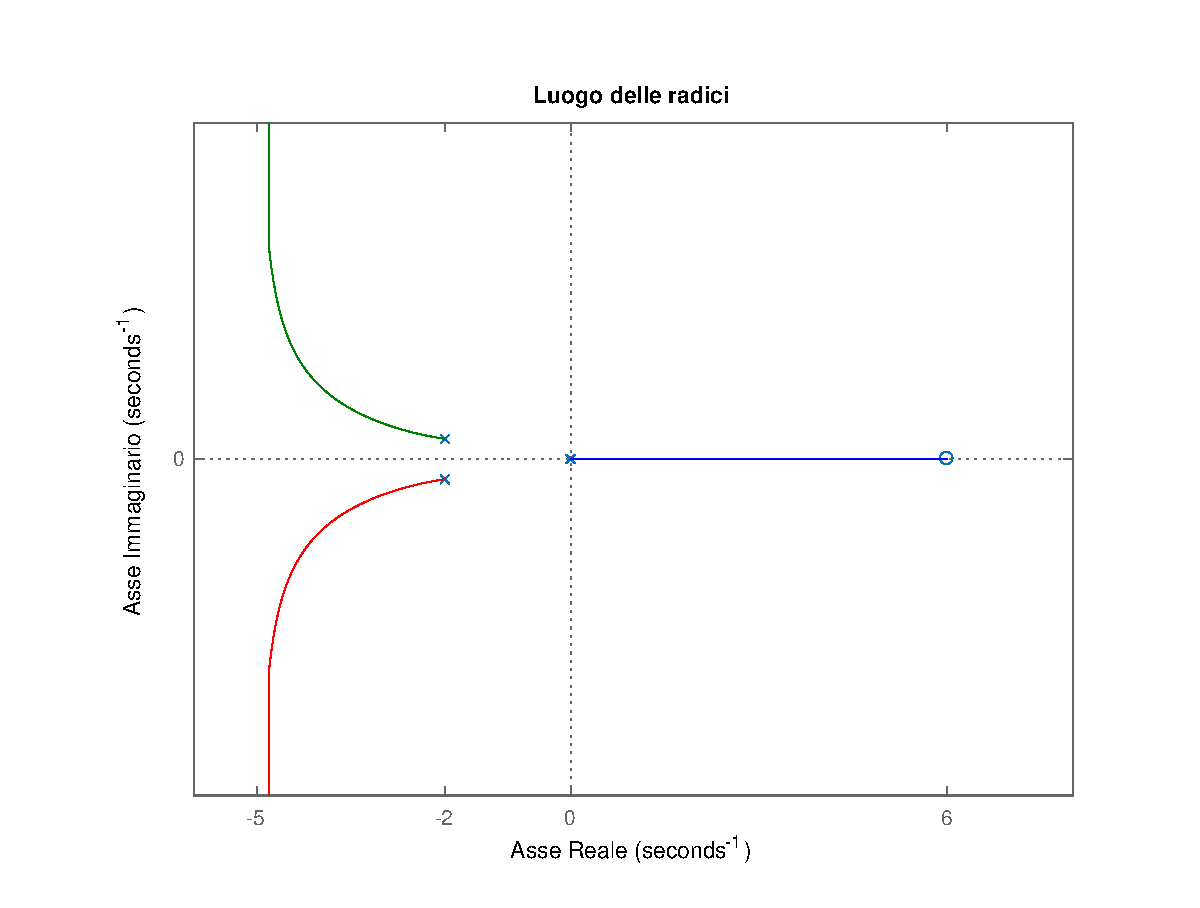
\includegraphics[scale=.5]{mod1/assets/rl_ex313}
	\caption{per \(k>0\)}
\end{figure}

\begin{itemize}
	\item \emph{Punti di singolarità}:
		\begin{itemize}
			\item poli: \(\bigl\{-2\pm\jmath3,0\bigr\}\)
			\item zeri: \(\bigl\{6\bigr\}\)
		\end{itemize}
	\item \emph{Asintoti}:
		\[
			\sigma_a = \frac{-4\pm\jmath3-6}{2} = -5 \qquad
			\theta_a = \frac{\Bigl(2\cdot\bigl[0,1\bigr]+1\Bigr)\pi}{2} = \Bigl[\frac{\pi}{2},\frac{3}{2}\pi\Bigr]
		\]
	\item \emph{Stabilità}:
		\[\begin{cases}
			k=0\colon & \text{sistema \emph{semplicemente stabile}} \\
			k>0\colon & \text{sistema \emph{instabile} con 1 polo instabile}
		\end{cases}\]
\end{itemize}

\paragraph{Soluzione per \(k<0\)}

\begin{figure}
	\centering
	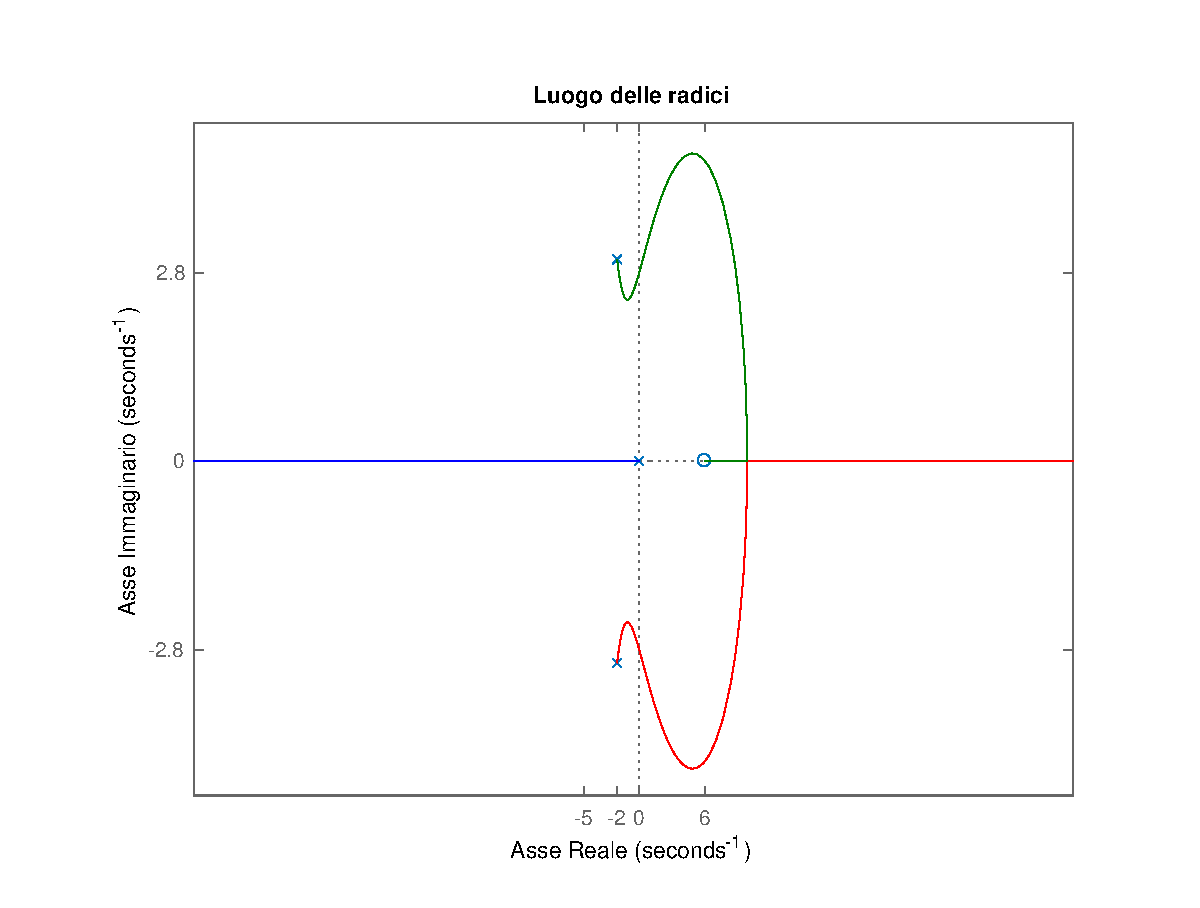
\includegraphics[scale=.5]{mod1/assets/rl_ex313n}
	\caption{per \(k<0\)}
\end{figure}

\begin{itemize}
	\item \emph{Asintoti}:
		\[
			\sigma_a = -5 \qquad
			\theta_a = \frac{2\cdot\bigl[0,1\bigr]\pi}{2} = \bigl[0,\pi\bigr]
		\]
	\item \emph{Punti doppi}:
		\[
			k = -\frac{s\bigl((s+2)^2+9\bigr)}{s-6} \quad
			\text{per } s \in (6,+\infty)
		\]
		\[\begin{array}{rr}
			\toprule
			     s &         k \\
			\midrule
			     8 &      -436 \\
			\bm{9} & \bm{-390} \\
			    10 &      -382.5 \\
			\bottomrule
		\end{array}\]
		Per \(s=9\) si ha un punto doppio di \emph{confluenza}.
	\item \emph{Angoli di partenza} per \(s=-2\pm\jmath3\):
		\begin{align*}
			\varphi_- &= \angle(-2-\jmath3-6) -\angle(-2-\jmath3+2-\jmath3) -\angle(-2-\jmath3) = \\
				  &= \arctan{\frac{3}{8}} -\pi +\frac{\pi}{2} -\arctan{\frac{3}{2}} +\pi = \\
				  &= \frac{\pi}{2} +0.359 -0.983 = \SI{0.946}{\radian} \\
			\varphi_+ &= \angle(-2+\jmath3-6) -\angle(-2+\jmath3+2-\jmath3) -\angle(-2+\jmath3) = \\
				  &= \arctan{-\frac{3}{8}} +\pi -\frac{\pi}{2} -\arctan{-\frac{3}{2}} -\pi = \\
				  &= -\frac{\pi}{2} -0.359 +0.983 = \SI{-0.946}{\radian}
		\end{align*}
	\item \emph{Intersezioni con l'asse immaginario}:
		\[
			P(s) = s^3 +4s^2 +(13+k)s -6k
		\]
		\[\begin{array}{r|rr}
			s^3 & 1 & 13+k \\
			s^2 & 4 & -6k  \\
			s^1 & 26+5k    \\
			s^0 & -6k
		\end{array}\]
		Per \(k = -\frac{26}{5}\) si ha \(4s^2+\frac{4\cdot39}{5}=0 \rightarrow s=\pm\jmath\sqrt{\frac{39}{5}}\).
	\item \emph{Stabilità}:
		\[\begin{cases}
			k < -\frac{26}{5}\colon & \text{sistema \emph{instabile} con 2 poli instabili} \\
			k = -\frac{26}{5}\colon & \text{sistema \emph{semplicemente stabile}} \\
			-\frac{26}{5} < k < 0\colon & \text{sistema \emph{asintoticamente stabile}}
		\end{cases}\]
\end{itemize}

\exercise{}
Sia data la seguente funzione di trasferimento
\[
	G(s) = \frac{s-1}{(s+1)^4}
\]
Determinare il luogo delle radici per \(k>0\).

\paragraph{Soluzione}

\begin{figure}[ht]
	\centering
	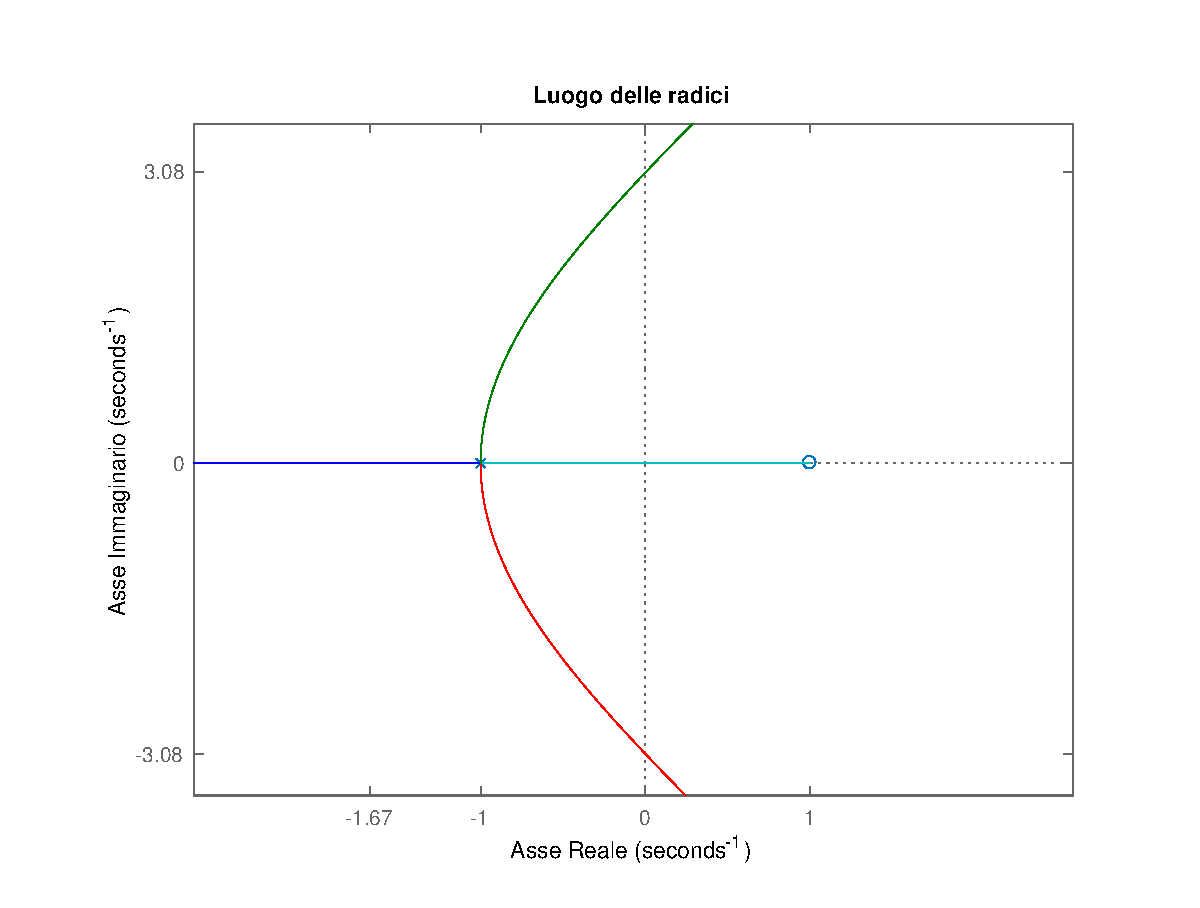
\includegraphics[scale=.6]{mod1/assets/rl_ex314}
\end{figure}

\begin{itemize}
	\item \emph{Punti di singolarità}:
		\begin{itemize}
			\item poli: \(\bigl\{-1\,[\times 4]\bigr\}\)
			\item zeri: \(\bigl\{1\bigr\}\)
		\end{itemize}
	\item \emph{Asintoti}:
		\[
			\sigma_a = \frac{4(-1)-1}{3} = -\frac{5}{3} \qquad
			\theta_a = \frac{\Bigl(2\cdot\bigl[0,1,2\bigr]+1\Bigr)\pi}{3} = \Bigl[\frac{\pi}{3},\pi,\frac{5}{3}\pi\Bigr]
		\]
	\item \emph{Intersezioni con l'asse immaginario}:
		\[
			P(s) = (s+1)^4 +ks -k = s^4+4s^3+6s^2+(4+k)s+1-k
		\]
		\[\begin{array}{r|rrr}
			s^4 & 1 & 6 & 1-k \\
			s^3 & 4 & 4+k \\
			\bm{s^2} & 20-k & 4-4k \\
			s^1 & \bm{-k^2+32k+64} \\
			s^0 & \bm{1-k}
		\end{array}\]
		Considerando
		\begin{align*}
			& k^2-32k-64=0 \\
			\rightarrow & k_1 = 16+8\sqrt{5} \\
			\rightarrow & (20-16-8\sqrt{5})s^2 +4-4(16+8\sqrt{5}) =0 \\
			\rightarrow & s=\pm\jmath\sqrt{\frac{15+8\sqrt{5}}{1-2\sqrt{5}}}
		\end{align*}
		Si nota inoltre che per \(k=1\) il sistema è \emph{semplicemente stabile}.
	\item \emph{Stabilità}:
		\[\begin{cases}
			0 \leq k < 1\colon & \text{sistema \emph{asintoticamente stabile}} \\
			k = 1\colon & \text{sistema \emph{semplicemente stabile}} \\
			1 < k \leq 16+8\sqrt{5}\colon & \text{sistema \emph{instabile} con 1 polo instabile} \\
			k > 16+8\sqrt{5}\colon & \text{sistema \emph{instabile} con 3 poli instabili}
		\end{cases}\]
\end{itemize}

\exercise{}
Sia data la seguente funzione di trasferimento:
\[
	G(s) = \frac{s+z}{s+p}
\]
Determinare \(z,p\) tale che il sistema sia asintoticamente stabile.

\paragraph{Soluzione}
Il sistema per poter esistere deve esser tale che \(p\neq0\).
Per \(p<0\) si hanno poli instabili, per \(p>0\) invece poli stabili, ovvero con
\(\Re s<0\).
Se \(z<0\), il sistema diventerebbe instabile ad un certo valore \(k\).

Quindi il sistema è essere asintoticamente stabile quando
\[
	z,p > 0
\]

\exercise{Appello Gennaio 2017}
\begin{center}\begin{tikzpicture}[auto,node distance=2cm,>=latex']
	\node [input] (U) {};
	\node [sum,right of=U] (sum) {};
	\node [block,right of=sum,node distance=1.5cm] (GC) {\(G_C(s)\)};
	\node [block,right of=GC] (GP) {\(G_P(s)\)};
	\node [output,right of=GP] (Y) {};
	\draw [->] (U) -- node[pos=0] {\(U(s)\)} (sum);
	\draw [->] (sum) -- (GC);
	\draw [->] (GC) -- node[pos=0.5,name=sym] {} (GP);
	\draw [->] (GP) -- node[pos=0.5,name=retro] {\(Y(s)\)} (Y);
	\node [block,below of=sym,node distance=1.5cm] (H) {\(H(s)\)};
	\draw [->] (retro) |- (H);
	\draw [->] (H) -| node[pos=0.9] {\(-\)} (sum);
\end{tikzpicture}\end{center}

\subsubsection{
Siano \(\displaystyle G_P(s) = \frac{s+1}{s(s-5)(s+5)}\) e \(H(s) = 1\). \\
Supponendo \(G_C(s)=k\), si tracci e si orienti il luogo delle radici del sistema complessivo per \(k>0\) e \(k<0\), determinando i punti del luogo sull'asse reale, il centroide e gli asintoti, i punti doppi e i punti di incontro con l'asse immaginario con i corrispondenti valori di \(k\), ove presenti.
}

\paragraph{Soluzione per \(k>0\)}
\begin{itemize}
	\item Punti di singolarità: \begin{itemize}
		\item poli: \(\set{-5,0,5}\)
		\item zeri: \(\set{-1}\)
	\end{itemize}
	\item Mappa poli-zeri e luogo delle radici:
		\begin{center}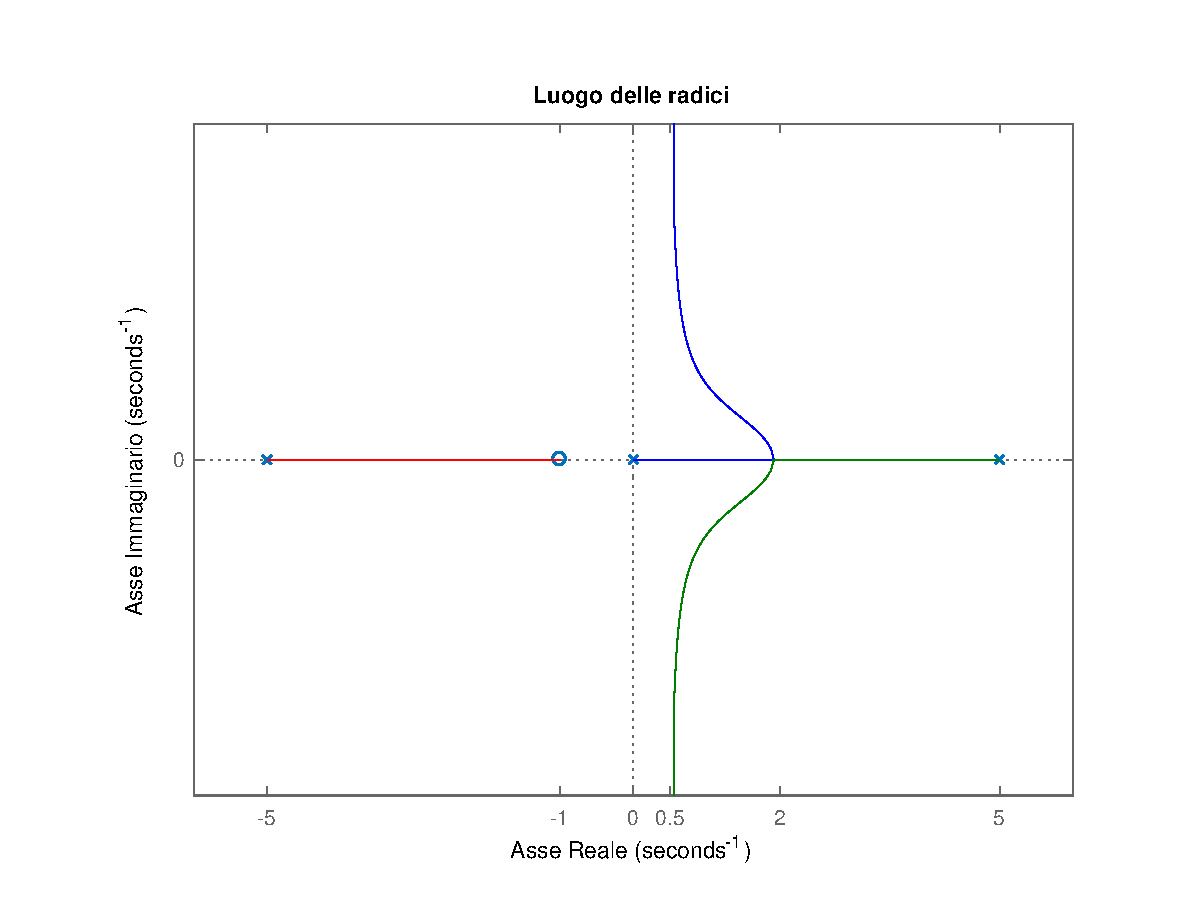
\includegraphics[scale=.5]{mod1/assets/rl_ex316.eps}\end{center}
	\item Asintoti: \begin{itemize}
		\item \(\displaystyle \sigma_a = \frac{0+5-5+1}{2} = \frac{1}{2}\)
		\item \(\displaystyle \theta_a = \frac{\qty(2\qty[0,1]+1)\pi}{2} = \qty[\frac{\pi}{2},\frac{3}{2}\pi]\)
	\end{itemize}
	\item Punti doppi: ne prevedo uno in \(\qty(0,5)\). Uso la \emph{tabella di taratura}:
		\[\begin{array}{rr}
			\toprule
			s & k \\
			\midrule
			1.5 & 13.65 \\
			\bm{2} & \bm{14} \\
			2.5 & 13.39 \\
			\bottomrule
		\end{array}\]
		Quindi per \(s=2\) si ha un punto di \emph{emergenza}.
	\item Intersezioni con l'asse immaginario: per \(k=0\) si ha un polo nell'origine.
\end{itemize}

\paragraph{Soluzione per \(k<0\)}
\begin{itemize}
	\item Mappa poli-zeri e luogo delle radici:
		\begin{center}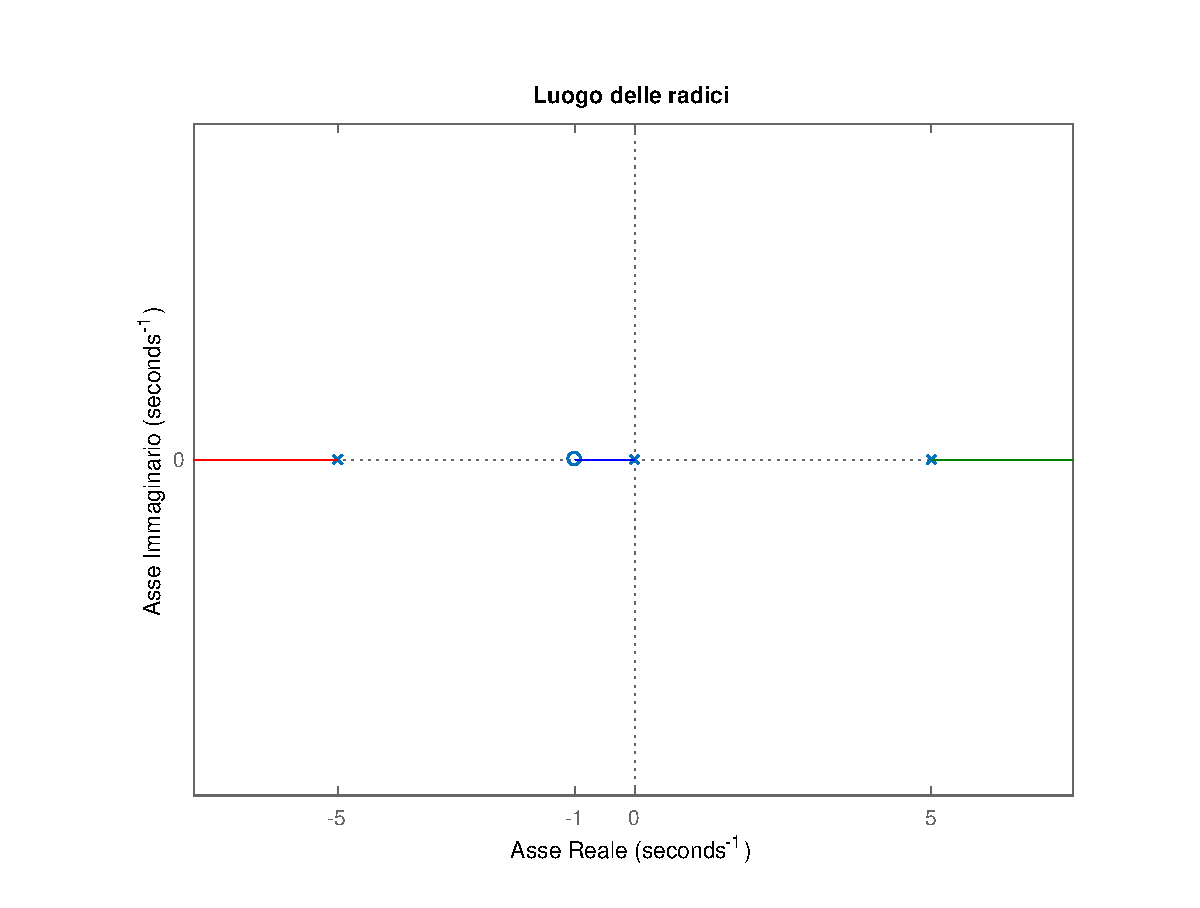
\includegraphics[scale=.5]{mod1/assets/rl_ex316n.eps}\end{center}
	\item Intersezioni con l'asse immaginario: per \(k=0\) si ha un polo nell'origine.
\end{itemize}

\subsubsection{
Sempre nell'ipotesi \(G_C(s)=k\), si discuta la stabilità del sistema in anello chiuso al variare del parametro \(k>0\) e \(k<0\), specificando per quali valori è rispettivamente asintoticamente stabile, semplicemente stabile, o instabile (in caso di instabilità si precisi il numero di poli instabili).
}

\begin{itemize}
	\item Per \(k=0\) il sistema è \emph{instabile} con 1 polo a parte reale positiva e un polo nell'origine;
	\item per \(k>0\) il sistema è \emph{instabile} con 2 poli a parte reale positiva;
	\item per \(k<0\) il sistema è \emph{instabile} con 1 polo a parte reale positiva.
\end{itemize}

\subsubsection{Determinare il valore di \(k\) per cui esiste un polo in anello chiuso di valore \(s=-3\)}

\[k = -\frac{1}{G(-3)} = 24\]

\subsubsection{Per il valore di \(k\) determinato, individuare sul luogo la porzione dei rami in cui sono posizionati gli altri due poli.}

Dato che per \(s\approx2\), \(k\approx14\), gli altri due poli devono per forza trovarsi dopo il punto di emergenza, in direzione per gli asintoti.

\exercise{}
\[kG(s) = k\frac{(s+1)(s+2)}{s^3(s^2+2s+2)}\]

\subsubsection{Soluzione per \(k>0\)}
\begin{itemize}
	\item Punti di singolarità: \begin{itemize}
		\item poli: \(\set{0 \qty[\times 3], -1\pm\jmath}\)
		\item zeri: \(\set{-2,-1}\)
	\end{itemize}
	\item Mappa poli-zeri e luogo delle radici:
		\begin{center}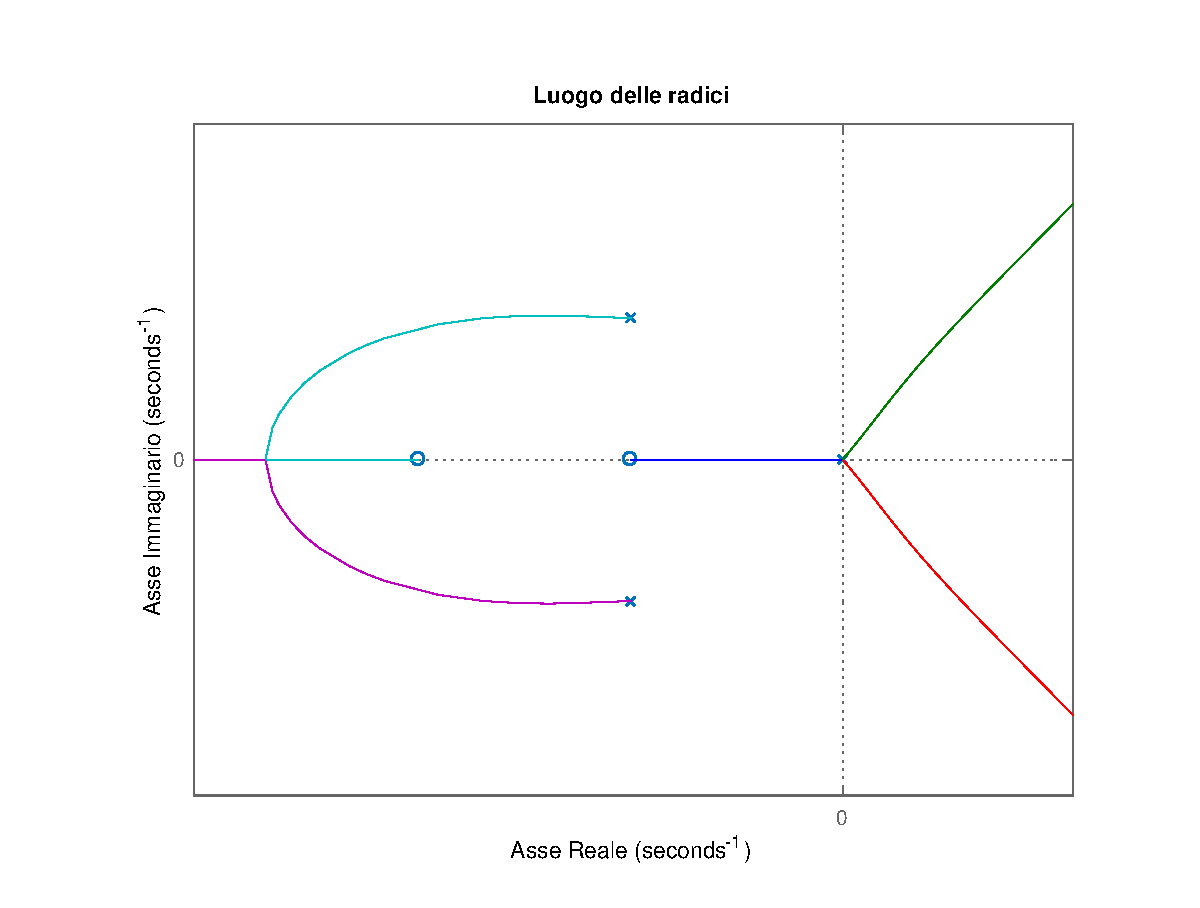
\includegraphics[scale=.5]{mod1/assets/rl_ex317.eps}\end{center}
	\item Asintoti: \begin{itemize}
		\item \(\displaystyle \sigma_a = \frac{-1+\jmath-1-\jmath+2+1}{3} = \frac{1}{3}\)
		\item \(\displaystyle \theta_a = \frac{\qty(2\qty[0,1,2]+1)\pi}{3} = \qty[\frac{\pi}{3},\pi,\frac{5}{3}\pi]\)
	\end{itemize}
	\item Punti doppi: ne prevedo uno in \((-\infty,2)\). Utilizzo la \emph{tabella di taratura}
		\[\begin{array}{rr}
			\toprule
			s & k \\
			\midrule
			-2.5 & 67.708 \\
			\bm{-3} & \bm{67.5} \\
			-3.5 & 82.89 \\
			\bottomrule
		\end{array}\]
		Quindi per \(s=-3\) si ha un punto di \emph{confluenza}.
	\item Angoli di partenza dei poli complessi e coniugati:
		\begin{align*}
			\varphi_+ &= \pi + \angle(-1+\jmath+2) + \angle(-1+\jmath+1) -3\angle(-1+\jmath) -\angle(-1+\jmath+1+\jmath) = \\
			&= \pi +\angle(1+\jmath) +\angle(\jmath) -3\angle(-1+\jmath) -\angle(2\jmath) = \\
			&= \pi + \frac{\pi}{4} + \frac{\pi}{2} -3\qty(-\frac{\pi}{4}+\pi) -\frac{\pi}{2} = -2\pi+\pi = -\pi \\
			\varphi_- &= \pi
		\end{align*}
	\item Stabilità: \begin{itemize}
			\item per \(k=0\) il sistema è \emph{instabile} con 3 poli nell'origine
			\item per \(k>0\) il sistema è \emph{instabile} con 2 poli instabili
		\end{itemize}
\end{itemize}

\subsubsection{Soluzione per \(k<0\)}
\begin{itemize}
	\item Mappa poli-zeri e luogo delle radici:
		\begin{center}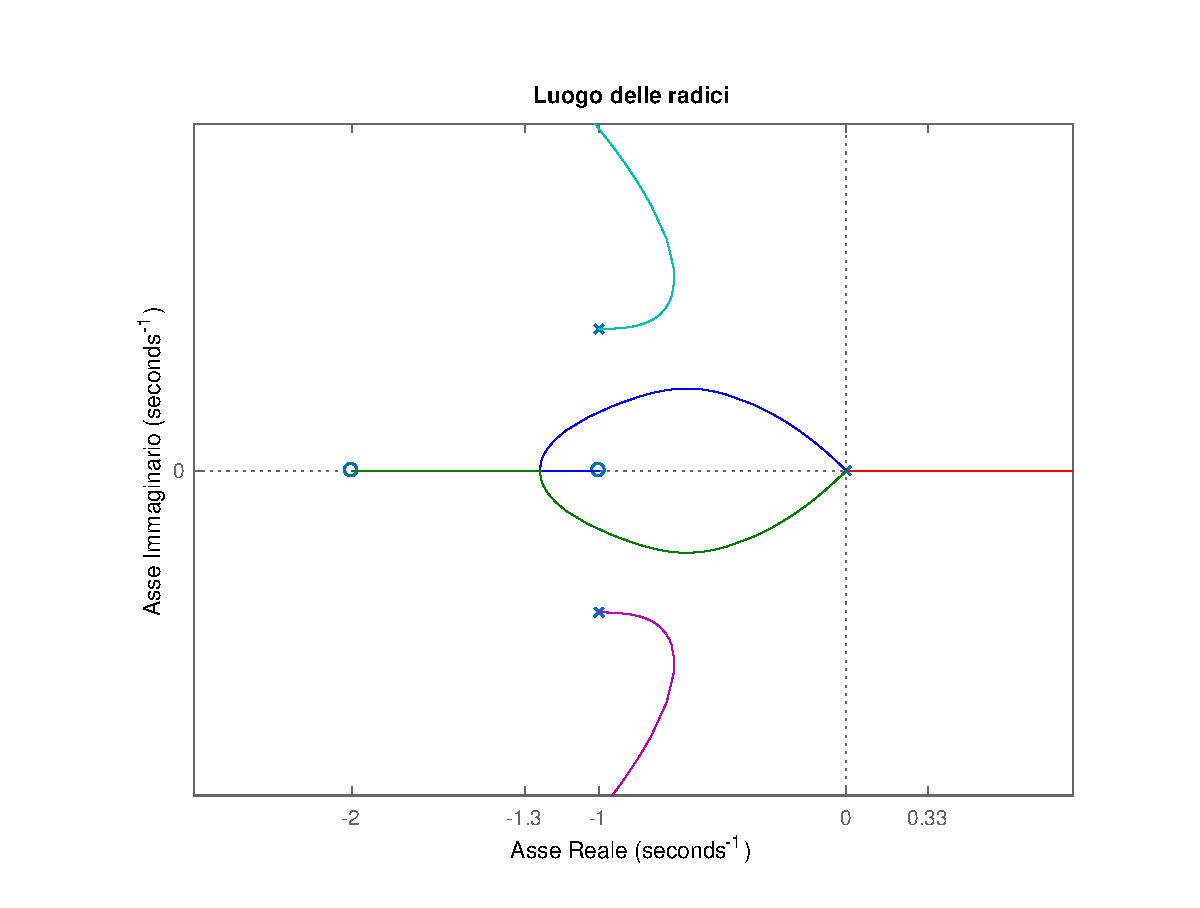
\includegraphics[scale=.5]{mod1/assets/rl_ex317n.eps}\end{center}
	\item Asintoti: \(\displaystyle \theta_a = \frac{2[0,1,2]\pi}{3} = \qty[0,\frac{2}{3}\pi,\frac{4}{3}\pi]\)
	\item Angoli di partenza dei poli complessi e coniugati: \(\varphi_+ = 0,\; \varphi_- = 0\)
	\item Punti doppi: mi aspetto un punto doppio in \((-2,-1)\). Ricorro alla \emph{tabella di taratura}:
		\[\begin{array}{rr}
			\toprule
			s & k \\
			\midrule
			-1.5 & -97.87 \\
			\bm{-1.3} & \bm{-65.8} \\
			-1.1 & -80 \\
			\bottomrule
		\end{array}\]
		Quindi si ha un punto di \emph{confluenza} per \(s=-1.3\).
	\item Stabilità: per \(k<0\) il sistema è \emph{instabile} con 1 polo instabile.
\end{itemize}